\ExerciseGroupsStart
\ExerciseSection

\begin{enumerate}
\def\labelenumi{\arabic{enumi})}
\item
  Let G be a discrete subgroup of rank p in \(R^{n}\) and let \((a_{i})_{1\leqslant i\leqslant p}\) be a free system of p points of G. The proof of Theorem 1 of no. 1 shows that G is a subgroup of the group generated by the p points \(d^{-1}a_{i}\) , where d is some integer. Show, without using Theorem 1, that there exists a free system of p points \(b_{i}=\sum_{j=1}^{p}b_{ij}a_{j}\) of G such that, if \(x_{i}=\sum_{j=1}^{p}x_{ij}a_{j}\quad(\mathrm{I}\leqslant i\leqslant p)\) is any free system of p points of G, we have \(|\det(x_{ij})|\geqslant|\det(b_{ij})|>0\) . Hence give a proof of Theorem 1 which does not rest on the theory of invariant factors, by showing that the \(b_{i}\) generate G. (Argue by contradiction: if \(z=\sum_{i=1}^{p}z_{i}b_{i}\in G\) and one of the \(z_{i}\) is not an integer, there exists a point \(u=\sum_{i=1}^{p}u_{i}b_{i}\) of the group generated by z and the \(b_{i}\) such that \(o<u_{i}<1\) for some index i, and hence obtain a contradiction.)
\item
  Let G be a discrete subgroup of \(R^{n}\) . If G is the direct sum of two subgroups H and K, then the intersection of the vector subspaces generated by H and K consists only of o, and the rank of G is therefore equal to the sum of the ranks of H and K (observe that, for every discrete subgroup G of \(R^{n}\) , the vector subspace of \(R^{n}\) generated by G is canonically isomorphic to \(G \otimes_{Z} R\) ).
\item
  Let G be a discrete subgroup of \(R^{n}\) . For a subgroup H of G to be a direct summand of G it is necessary and sufficient that \(H = V \cap G\) where V is a vector subspace of \(R^{n}\) (for necessity, use Exercise 2; for sufficiency, note that H is also the intersection of G and the vector subspace generated by H).
\item
  Let H and K be two discrete subgroups of \(R^{n}\) such that \(H + K\) is a closed subgroup. Show that \(H + K\) is then discrete and that \(r(\mathrm{H}) + r(\mathrm{K}) = r(\mathrm{H} \cap \mathrm{K}) + r(\mathrm{H} + \mathrm{K})\) . (Let V be the vector subspace of \(R^{n}\) generated by \(H \cap K\) ; split up H into the direct sum of \(V \cap H\) and a discrete group \(H_{1}\) , and K into the direct sum of \(V \cap K\) and a discrete group \(K_{1}\) , using Exercise 3; then show that the sum \(H_{1} + K_{1}\) is direct and use Exercise 2.)
\item
  Let G, \(G'\) be two closed subgroups of \(R^{n}\) such that \(G' \subset G\) , and let V (resp. \(V'\) ) be the largest vector subspace contained in G (resp. \(G'\) ). Show that there is a vector subspace W complementary to V such that G is the direct sum of V and the discrete group \(K = W \cap G\) , and such that \(G'\) is the direct sum of \(V \cap G'\) and \(K \cap G' = W \cap G'\) . (If U is a vector subspace complementary to \(V'\) , use Exercise 3 to show that the discrete group \(U \cap G'\) is the direct sum of \(U \cap V \cap G'\) and a discrete group \(K'\) , and take W to be a vector subspace containing \(K'\) .) Deduce that:
\end{enumerate}

\begin{enumerate}
\def\labelenumi{\alph{enumi})}
\tightlist
\item
  The quotient group \(G/G'\) is isomorphic to a product group of the form
\end{enumerate}

\[
\mathbf {R} ^ {p} \times \mathbf {T} ^ {q} \times \mathbf {Z} ^ {r} \times \mathbf {F},
\]

where F is a finite abelian group.

\begin{enumerate}
\def\labelenumi{\alph{enumi})}
\setcounter{enumi}{1}
\tightlist
\item
  Every closed subgroup and every Hausdorff quotient group of a group of the form \(R^{p} \times T^{q} \times Z^{r} \times F\) (F finite and abelian) are of the same form.
\end{enumerate}

\begin{enumerate}
\def\labelenumi{\arabic{enumi})}
\setcounter{enumi}{5}
\tightlist
\item
  Let H and K be two closed subgroups of \(R^{n}\) such that \(H + K\) is a closed subgroup.
\end{enumerate}

\begin{enumerate}
\def\labelenumi{\alph{enumi})}
\item
  Show that, if V (resp. W) is the largest vector subspace contained in H (resp. K), then \(V + W\) is the largest vector subspace contained in G, and therefore \(d(\mathrm{H}) + d(\mathrm{K}) = d(\mathrm{H} \cap \mathrm{K}) + d(\mathrm{H} + \mathrm{K})\) {[}note that the rational rank of \(\mathrm{G}/(\mathrm{V} + \mathrm{W})\) is finite and consequently that G cannot contain a line which is not contained in \(V + W\) {]}.
\item
  Let U be a subspace complementary to \(V + W\) , such that G is the direct sum of \(V + W\) and \(M = G \cap U\) , and such that \(H \cap K\) is the direct sum of \((V + W) \cap (H \cap K)\) and \(L = H \cap K \cap U\) (Exercise 5). Let \(H'\) (resp. \(K'\) ) be the subgroup of M consisting of the components of the points of H (resp. K) in the decomposition of G into the direct sum of \(V + W\) and M. Show that \(M = H' + K'\) and that \(H' \cap K' = L\) .
\item
  If we put \(H'' = H \cap (V + W)\) and \(K'' = K \cap (V + W)\) , show that \(r(H'') + r(K'') = r(H'' \cap K'') + r(H'' + K'')\) (reduce to the case where \(V \cap W = \{o\}\) , and show that then \(H'' \cap K''\) is the direct sum of \(V \cap K''\) and \(W \cap H''\) .
\end{enumerate}

\(d\) ) Show that

\[
r (\mathrm{H}) + r (\mathrm{K}) = r (\mathrm{H} \cap \mathrm{K}) + r (\mathrm{H} + \mathrm{K})
\]

{[}use c) and Exercise 4, noting that \(r(\mathbf{H}) = r(\mathbf{H}') + r(\mathbf{H}'')\) and \(r(\mathbf{K}) = r(\mathbf{K}') + r(\mathbf{K}'' )\) {]}.

\begin{enumerate}
\def\labelenumi{\arabic{enumi})}
\setcounter{enumi}{6}
\item
  Let G be a closed subgroup of \(R^{n}\) and let H be a closed subgroup of G. Then G is the direct sum of H and another closed subgroup K if and only if H is the intersection of G and a vector subspace. (Use Exercise 5 for the necessity; to show sufficiency, apply Theorem 2 of no. 2 appropriately to G and H, and use Exercise 3).
\item
  \begin{enumerate}
  \def\labelenumii{\alph{enumii})}
  \tightlist
  \item
    Let H, K be two closed subgroups of \(R^{n}\) . Show that if \(r(\mathrm{H}) + r(\mathrm{K})\) is equal to \(r(\mathrm{H} \cap \mathrm{K}) + r(\mathrm{H} + \mathrm{K})\) , then \(H + K\) is closed in \(R^{n}\) . {[}Using Exercise 7 and the hypothesis given, reduce to the case where H, K and \(H \cap K\) all generate the same vector subspace; if V (resp. W) denotes the largest subspace contained in H (resp. K), show with the help of Exercise 5 that V is generated by \(V \cap K\) , and W is generated by \(W \cap H\) ; finally, split up \(H \cap K\) into the direct sum of \(H \cap K \cap (V + W)\) and a discrete group, by using Exercise 7.{]}
  \end{enumerate}
\end{enumerate}

\begin{enumerate}
\def\labelenumi{\alph{enumi})}
\setcounter{enumi}{1}
\item
  Deduce from a) and Exercise 6 that, if H and K are two closed subgroups of \(R^{n}\) such that \(H + K\) is a closed subgroup, then \(H^{*} + K^{*}\) is also a closed subgroup.
\item
  Deduce from b) that if H and K are two closed subgroups of \(R^{n}\) such that \(d(\mathrm{H}) + d(\mathrm{K}) = d(\mathrm{H} \cap \mathrm{K}) + d(\overline{\mathrm{H} + \mathrm{K}})\) , then the subgroup \(H + K\) is closed.
\end{enumerate}

\begin{enumerate}
\def\labelenumi{\arabic{enumi})}
\setcounter{enumi}{8}
\item
  Let G be a subgroup of \(R^{n}\) , not necessarily closed, of rank p, and let V be the largest vector subspace contained in \(\overline{G}\) . If V has dimension \(q \leqslant p\) , show that G is the direct sum of \(V \cap G\) and a discrete subgroup of rank p - q contained in a vector subspace complementary to V {[}note that, for each \(x \in \overline{G}\) , \((x + V) \cap G\) is dense in the linear variety \(x + V\) {]}.
\item
  Let \(a\) be a real number and \(n\) an integer \(>0\) , and consider the numbers \(x_{k} = ka - [ka] \in [0, \mathrm{I}[(\mathrm{I} \leqslant k \leqslant n + \mathrm{I})\) . If \(\mathbf{I}_h\) denotes the interval
\end{enumerate}

\[
\left[ \frac {h - \mathrm{I}}{n}, \frac {h}{n} \right] \quad (\mathrm{I} \leqslant h \leqslant n),
\]

show that there exist two distinct indices \(k, k'\) such that \(x_k\) and \(x_{k'}\) belong to the same interval \(I_h\) (for a suitable value of \(h\) ). Deduce that there exist two integers \(p, q\) such that \(1 \leqslant p \leqslant n\) and \(|pa - q| \leqslant 1 / n\) .

\begin{enumerate}
\def\labelenumi{\Roman{enumi})}
\setcounter{enumi}{1}
\tightlist
\item
  Let \(\boldsymbol{a}_i = (a_{ij})\) ( \(1 \leqslant i \leqslant m\) , \(1 \leqslant j \leqslant n\) ) be \(m\) points of \(\mathbf{R}^n\) and let \(q\) be an integer \(>0\) . For each point \(\boldsymbol{k} = (k_i)\) ( \(1 \leqslant i \leqslant m\) ) of \(\mathbf{R}^m\) with integer coordinates, not all zero, satisfying the inequalities \(0 \leqslant k_i \leqslant q\) , consider the point \(x_k = (x_{j,k})\) ( \(1 \leqslant j \leqslant n\) ) of \(\mathbf{R}^n\) , all of whose coordinates belong to {[}o, i{[} and which is congruent mod \(Z^n\) to \(\sum_{i=1}^{m} k_i a_i\) , i.e., the point with coordinates
\end{enumerate}

\[
x _ {j, k} = \sum_ {i = 1} ^ {m} k _ {i} a _ {i j} - \left[ \sum_ {i = 1} ^ {m} k _ {i} a _ {i j} \right].
\]

If \(p\) is the smallest integer such that \(q + 1 \geqslant p^{n/m}\) , show that there are two distinct points \(k, k'\) such that \(x_k\) and \(x_{k'}\) both belong to the same cube of side \(1/p\) (same method as Exercise 10). Deduce that there exist \(m\) integers \(p_i\) , not all zero, and \(n\) integers \(r_j\) ( \(1 \leqslant j \leqslant n\) ) such that \(0 \leqslant p_i \leqslant q\) for \(1 \leqslant i \leqslant m\) , and

\[
\left| \sum_ {i = 1} ^ {m} p _ {i} a _ {i j} - r _ {j} \right| \leqslant \frac {\mathrm{I}}{p} \quad (\mathrm{I} \leqslant j \leqslant n).
\]

Use this result to give another proof of Proposition 2 of no. 1 (the ``pigeon-hole principle'').

\begin{enumerate}
\def\labelenumi{\arabic{enumi})}
\setcounter{enumi}{11}
\tightlist
\item
  For each pair of real numbers \((\theta, \beta)\) there exists an infinite number of triples \((p, q, r)\) of integers such that \(r > 0\) , \(|q| \leqslant \frac{1}{2} r\) and
\end{enumerate}

\[
- \frac {\mathrm{I}}{r} <   \theta q + p - \beta <   \frac {\mathrm{I}}{r}.
\]

{[}If \(m, n\) are two integers such that \(|n\theta - m| < 1/n\) (Exercise 10), take \(r = n\) and choose \(p, q\) so that \(pn + qm\) differs from \(n\beta\) by less than \(1/2\) {]}.

\begin{enumerate}
\def\labelenumi{\arabic{enumi})}
\setcounter{enumi}{12}
\tightlist
\item
  The Farey series of order \(n\) ( \(n\) an integer \(>0\) ) is the set \(F_n\) of rational numbers \(p/q\) in their lowest terms such that \(0 \leqslant p \leqslant q \leqslant n\) , arranged in increasing order (i.e., the Farey series is a sequence).
\end{enumerate}

\begin{enumerate}
\def\labelenumi{\alph{enumi})}
\item
  Show that if two rational numbers \(r = p / q\) , \(r' = p' / q'\) are such that \(p'q - pq' = \pm 1\) , then every pair of integers \((p'', q'')\) can be expressed in the form \(p'' = px + p'y\) , \(q'' = qx + q'y\) where \(x\) and \(y\) are integers. The fraction \(p'' / q''\) belongs to the closed interval with end-points \(r\) and \(r'\) if and only if \(x\) and \(y\) have the same sign.
\item
  Deduce from a) that if \(r = p / q\) and \(r' = p' / q'\) are two rational numbers in {[}0, 1{]} such that \(q > 0\) and \(q' > 0\) and \(qp' - pq' = \pm 1\) , then \(r\) and \(r'\) are consecutive elements in the sequence \(\mathbf{F}_n\) , where \(n = \max (q, q')\) . Furthermore, the smallest integer \(m\) such that the open interval with end-points \(r\) and \(r'\) contains a point of \(\mathbf{F}_m\) is \(m = q + q'\) , and there is only one point of \(\mathbf{F}_{q + q'}\) in this interval, namely the fraction \((p + p') / (q + q')\) .
\item
  Show that conversely, if \(r\) and \(r'\) are two consecutive elements of \(\mathbf{F}_n\) , we have \(p'q - pq' = \pm 1\) (use induction on \(n\) ).
\item
  Deduce from c) that, for each real number \(\theta \in [\mathrm{o},\mathrm{i}]\) and each integer \(n\geqslant \mathrm{i}\) , there is at least one fraction \(p / q\) in its lowest terms such that \(\mathrm{i}\leqslant q\leqslant n\) and \(|\theta -p / q|\leqslant \mathrm{i} / (n + \mathrm{i})q\) (cf.~Exercise 10).
\item
  If \(p / q\) is a fraction in its lowest terms such that \(|\theta - p / q| < 1 / q^2\) , then \(\theta\) belongs to the open interval whose end-points are the two terms of the Farey series \(\mathbf{F}_q\) consecutive to \(p / q\) .
\end{enumerate}

\begin{enumerate}
\def\labelenumi{\arabic{enumi})}
\setcounter{enumi}{13}
\tightlist
\item
  Let \(\varphi: \mathbf{R} \to \mathbf{T}\) be the canonical homomorphism; let \(\theta\) be an element of infinite order in \(\mathbf{T}\) and let \(\theta_0\) be an (irrational) real number such that \(\varphi(\theta_0) = \theta\) . For each integer \(n > 0\) , let \(\mathbf{S}_n\) be the set of elements \(k\theta\) of \(\mathbf{T}\) for which \(\mathbf{i} \leqslant k \leqslant n\) , and for each interval \(\mathbf{I}\) of \(\mathbf{R}\) let \(\mathrm{N}(\mathbf{I}, n)\) be the number of elements of the set \(\mathbf{I} \cap \overline{\varphi}^1(\mathbf{S}_n)\) .
\end{enumerate}

\begin{enumerate}
\def\labelenumi{\alph{enumi})}
\item
  If we take \(\mathbf{I} = [\mathrm{o},\theta_0[\) , show that \(\mathrm{N(I,n)} = [n\theta_0]\) {[}note that \(\mathrm{N(I,n)}\) is then the number of pairs of integers \((x,y)\) such that \(\mathrm{i}\leqslant y\leqslant n\) and \(x\leqslant y\theta_0 < x + \theta_0]\) .
\item
  More generally, if we take \(\mathbf{I} = [\mathrm{o}, m\theta_0[, m\) being an integer, we have \(m. [(n - m)\theta_0] \leqslant \mathrm{N}(\mathrm{I}, n) \leqslant m. [n\theta_0]\) (same method).
\item
  Deduce that, if I is any interval, the number \(\mathrm{N}(\mathrm{I}, n)/n\) tends to a limit equal to the length of I, as \(n \to +\infty\) . (Prove the result first when I is of the form \([m\theta_{0} + a, m'\theta_{0} + a']\) , where \(m, m', a\) and \(a'\) are integers, by using b); then pass to the general case by approximating to the endpoints of I by numbers of the form \(m\theta_{0} + a\) .) {[}``Equipartition of the sequence \((k\theta) \mod 1\)''.{]}
\end{enumerate}

* 15) Let I be a closed cube in \(\mathbf{R}^n\) with side \(2\pi\) . Map each point \(x = (x_i)\) of I to the point \(y = (y_j)\) of \(\mathbf{R}^{n+1}\) such that

\[
\begin{array}{l} y _ {1} = \sin x _ {1} \\ y _ {2} = (2 + \cos x _ {1}) \sin x _ {2} \end{array}
\]

\[
y _ {p} = \left(2 ^ {p - 1} + \sum_ {k = 1} ^ {p - 1} 2 ^ {p - k - 1} \cos x _ {p - k} \cos x _ {p - k + 1} \dots \cos x _ {p - 1}\right) \sin x _ {p} \quad (2 \leqslant p \leqslant n)
\]

\[
y _ {n + 1} = \sum_ {k = 1} ^ {n - 1} 2 ^ {p - k - 1} \cos x _ {n - k} \cos x _ {n - k + 1} \dots \cos x _ {n}.
\]

Show that the image of I under this mapping is homeomorphic to \(T^{n}\) (proof by induction on n: observe that \(y_{p}\) has the sign of \(\sin x_{p}\) for \(2 \leqslant p \leqslant n\)). If n=2, the subset of \(R^{3}\) so defined is called a torus of revolution.*

¶ 16) Let G be a subgroup of \(\mathbf{R}^n\) which contains a compact connected subset K such that the affine linear variety generated by K is of dimension \(p\) . Show that G contains a vector subspace of dimension \(p\) . {[}Proof by induction on \(n\) , using Exercise 10 c) of Chapter VI, § 1.{]}

\(\mathbb{J}\) 17) Let \(\mathbf{E}\) be the product \((\mathbf{Q}_p)^n\) of \(n\) factors equal to the field \(\mathbf{Q}_p\) of \(p\) -adic numbers (Chapter III, § 6, Exercise 23), endowed with the topological group structure which is the product of the additive topological structures of the factors \(\mathbf{Q}_p\) , and with its \(n\) -dimensional vector space structure over the field \(\mathbf{Q}_p\) . If \(v\) denotes the additive \(p\) -adic valuation on \(\mathbf{Q}_p\) , put \(|x|_p = p^{-v_p(x)}\) for all \(x \neq 0\) in \(\mathbf{Q}_p\) , and \(|o|_p = 0\) ; and put \(||x|| = \sup |x_i|_p\) for all \(x = (x_i)_{1 \leqslant i \leqslant n} \in \mathbf{E}\) (cf.~Chapter IX, § 3, nos. 2 and 3).

\begin{enumerate}
\def\labelenumi{\alph{enumi})}
\tightlist
\item
  A subset \(\mathbf{A}\) of \(\mathbf{E}\) is relatively compact if and only if
\end{enumerate}

\[
\sup _ {\mathbf {x} \in \mathbf {A}} | | \mathbf {x} | | <   + \infty .
\]

{[}Note that \(v_{p}\) is a continuous mapping of \(\mathbf{Q}_p\) into \(\mathbf{Z}\) (with the discrete topology).{]}

\begin{enumerate}
\def\labelenumi{\alph{enumi})}
\setcounter{enumi}{1}
\item
  If \(\mathbf{G}\) is a closed subgroup of \(\mathbf{E}\) , then \(\mathbf{G}\) is a topological module over the ring \(\mathbf{Z}_p\) of \(p\) -adic integers (if \(\boldsymbol{x} \in \mathbf{G}\) , we have \(n\boldsymbol{x} \in \mathbf{G}\) for all \(n \in \mathbf{Z}\) , and \(\mathbf{Z}\) is dense in \(\mathbf{Z}_p\) ).
\item
  If K is a compact subgroup of E, there exists a free system of \(m \leqslant n\) points \(a_{i}\) ( \(i \leqslant i \leqslant m\) ) of E, such that K is the direct sum of the m groups \(Z_{p}.a_{i}\) . {[}Use a) to show that, if \((\boldsymbol{e}_{j})_{1 \leqslant j \leqslant n}\) is the canonical base of E, there is an integer \(k \in Z\) such that K is contained in the direct sum of the n groups \(Z_{p}.p^{k}\boldsymbol{e}_{j}\) ; then apply the theory of modules over a principal ideal ring.{]}
\item
  If G is a closed (but not compact) subgroup of E, then G contains a vector subspace of dimension 1, \(Q_{p} \cdot a\) with \(a \neq 0\) . {[}Let C be the compact subset of E consisting of all points \(x \in E\) such that \(\|x\| = 1\) ; show that \(G \cap C\) contains a sequence of points \((\boldsymbol{x}_{r})_{r \in \mathbb{N}}\) such that \(p^{-r}x_{r} \in G\) , and take a to be a cluster point of this sequence.{]}
\item
  Let G be a closed subgroup of E, let V be the largest vector subspace contained in G and let W be a vector subspace complementary to V; show that \(W \cap G\) is compact and that G is the direct sum of V and \(W \cap G\) (argue as in Theorem 2 of no. 2).
\end{enumerate}

\(f)\) Given a subgroup \(\mathbf{G}\) of \(\mathbf{E}\) , let \(\mathbf{G}^*\) denote the set of all \(\boldsymbol{u} = (u_i) \in \mathbf{E}\) such that

\[
(u | x) = \sum_ {i = 1} ^ {n} u _ {i} x _ {i}
\]

belongs to \(\mathbf{Z}_p\) for all \(x = (x_i) \in \mathbf{G}\) . Show that \(\mathbf{G}^*\) is closed in \(\mathbf{E}\) , that \((\overline{\mathbf{G}})^* = \mathbf{G}^*\) and that \((\mathbf{G}^*)^* = \overline{\mathbf{G}}\) .

\begin{enumerate}
\def\labelenumi{\alph{enumi})}
\setcounter{enumi}{6}
\tightlist
\item
  State and prove the analogues of Exercises 2 to 8 inclusive for closed subgroups of E. In particular, every closed subgroup and every Hausdorff quotient group of a group of the form
\end{enumerate}

\[
(\mathbf {Q} _ {p}) ^ {r} \times (\mathbf {Q} _ {p} / \mathbf {Z} _ {p}) ^ {s} \times (\mathbf {Z} _ {p}) ^ {t} \times \mathbf {F}
\]

(where F is the product of a finite number of cyclic groups of p-power order) is a group of the same form.

\ExerciseSection

\begin{enumerate}
\def\labelenumi{\arabic{enumi})}
\tightlist
\item
  Let \(\varphi\) be the canonical homomorphism of \(\mathbf{R}^n\) onto \(\mathbf{T}^n\) and let \(u\) be a linear mapping of \(\mathbf{R}^m\) into \(\mathbf{R}^n\) . For \(\varphi \circ u\) to be a strict morphism of \(\mathbf{R}^m\) into \(\mathbf{T}^n\) it is necessary and sufficient that either:
\end{enumerate}

\begin{enumerate}
\def\labelenumi{\alph{enumi})}
\item
  \(\overline{u}^1 (\mathbf{Z}^n)\) is of rank \(m\) ; or
\item
  \(u(\mathbf{R}^m)\cap \mathbf{Z}^n\) is of rank equal to the dimension of \(u(\mathbf{R}^m)\) .
\end{enumerate}

\begin{enumerate}
\def\labelenumi{\arabic{enumi})}
\setcounter{enumi}{1}
\item
  Show that the only continuous homomorphism of the additive topological group \(Q_{p}\) of p-adic numbers (Chapter III, § 6, Exercises 23 et seq.) into the additive group R is the zero mapping.
\item
  Every \(p\) -adic number \(x\) (Exercise 2) can be written in the form \(\sum_{-\infty}^{+\infty} \alpha_k p^k\) where the \(\alpha_k\) are rational integers, those of index \(k < 0\) being zero for all but a finite number of values of the index \(k\) . Moreover, if \(\sum_{-\infty}^{+\infty} \alpha_k p^k = \sum_{-\infty}^{+\infty} \beta_k p^k\) , the rational numbers \(\sum_{-\infty}^{-1} \alpha_k p^k\) and \(\sum_{-\infty}^{-1} \beta_k p^k\) are congruent mod 1. Let \(\varphi_p(x)\) be the class mod 1 of the rational number \(\sum_{-\infty}^{-1} \alpha_k p^k\) .\\
\end{enumerate}

\begin{enumerate}
\def\labelenumi{\alph{enumi})}
\tightlist
\item
  Show that \(\varphi_p\) is a continuous homomorphism of the topological group \(\mathbf{Q}_p\) into \(\mathbf{T}\) , and that for every continuous homomorphism \(f\) of \(\mathbf{Q}_p\) into \(\mathbf{T}\) there exists a unique \(a \in \mathbf{Q}_p\) such that \(f(x) = \varphi_p(ax)\) for all \(x \in \mathbf{Q}_p\) . {[}Note that the knowledge of the elements \(f(p^k)\) for \(k \leqslant 0\) determines \(f\) uniquely; show that each of these elements is the class mod 1 of a fraction whose denominator is a power of \(p\) ; hence show that there exists \(a \in \mathbf{Q}_p\) such that \(f(p^k) = \varphi_p(ap^k)\) for all \(k \leqslant 0\) .{]}\\
\item
  Show that, if \(\varphi: \mathbf{R} \to \mathbf{T}\) is the canonical homomorphism, then \(\varphi(x) = \sum_{p} \varphi_p(x)\) for all \(x \in \mathbf{Q}\) , the sum being over all prime numbers \(p\) (observe that all but a finite number of terms of this sum will be zero).
\end{enumerate}

¶ 4) a) Let G be a locally compact abelian group and let H be a subgroup of G isomorphic to \(\mathbf{R}^{p} \times \mathbf{T}^{q}\) where \(p, q\) are integers \(\geqslant 0\) ; suppose also that G/H is isomorphic to either R or T. Show that G is isomorphic to the product of H and a closed subgroup L isomorphic to G/H. {[}Apply Chapter V, § 3, Exercise 7 d), to obtain a continuous homomorphism \(f\) of R into G such that \(f(\mathbf{R}) \subset \mathbf{H}\) ; hence construct another continuous homomorphism \(g: \mathbf{R} \to \mathbf{G}\) such that \(f(t) - g(t) \in \mathbf{H}\) for all \(t \in \mathbf{R}\) and \(g(\mathbf{R}) \cap \mathbf{H} = \{e\}\) . Note that \(f(\mathbf{H})\) is a proper closed subgroup of R and that, for every element \(z \neq e\) in H, there exists a continuous homomorphism \(u\) of R into H such that \(u(1) = z\) .{]}

\begin{enumerate}
\def\labelenumi{\alph{enumi})}
\setcounter{enumi}{1}
\tightlist
\item
  Let G be a Hausdorff abelian topological group, let H be a closed subgroup of G isomorphic to \(R^{p} \times T^{q}\) , and suppose that there exists a surjective continuous homomorphism \(\varphi: R \to G/H\) . Show that there exists a continuous homomorphism \(f: R \to G\) such that \(f(\mathbf{R}) \cap \mathbf{H} = \{e\}\) and \(\mathbf{G} = \mathbf{H}. f(\mathbf{R})\) . {[}Reduce to case a) by considering the least upper bound on G of the given topology and the topology for which a funda-
\end{enumerate}

mental system of neighbourhoods of o is formed by the \(\overline{p}(\varphi(I))\) , where \(p:G\to G/H\) is the canonical mapping and I runs through a fundamental system of neighbourhoods of o in R; show that G is locally compact in this new topology (cf.~Chapter III, § 4, Exercise 10 e).{]}

\begin{enumerate}
\def\labelenumi{\alph{enumi})}
\setcounter{enumi}{2}
\tightlist
\item
  Give an example where the restriction of \(p\) to \(f(\mathbf{R})\) is not bicontinuous {[}cf.~§ 1, Exercise 2f){]}.
\end{enumerate}

\begin{enumerate}
\def\labelenumi{\arabic{enumi})}
\setcounter{enumi}{4}
\item
  Let G be a connected topological group and let H be a compact normal subgroup of G with no arbitrarily small subgroups (Chapter III, § 2, Exercise 30). Show that H is contained in the centre of G. (Observe that for s close to e in G, the image of H under \(x \rightarrow sxs^{-1}\) is arbitrarily close to e.)
\item
  Let \(\mathbf{G}\) be a topological group and let \(\mathbf{H}\) be a closed normal subgroup of \(\mathbf{G}\) , isomorphic to \(\mathbf{R}^n (n\geqslant 1)\) and such that \(\mathbf{G} / \mathbf{H}\) is abelian.
\end{enumerate}

\begin{enumerate}
\def\labelenumi{\alph{enumi})}
\item
  Suppose, moreover, that H contains no connected subgroup normal in G except for H itself and \(\{e\}\) , and that H is not contained in the centre of G. Given \(x_{0} \in G\) which does not commute with every element of H, show that, for every \(v \in H\) , there exists a unique \(u \in H\) such that \(x_{0}^{-1}ux_{0}u^{-1} = v\) . (Observe that in the additive notation in H the equation becomes \(u - x_{0}^{-1}ux_{0} = -v\) and that the continuous endomorphism \(u \to u - x_{0}^{-1}ux_{0}\) of H is a linear mapping of \(R^{n}\) into itself. Show that its kernel is a normal subgroup of G.) Furthermore, if \(f(u)\) is the unique \(u \in H\) such that \(x_{0}^{-1}ux_{0}u^{-1} = v\) , then f is a bicontinuous automorphism of H.
\item
  Under the hypotheses of a), show that the continuous mapping \(g: y \to (f(x_{0}^{-1}yx_{0}y^{-1}))^{-1}y\) of G into itself has as image the subgroup L of G consisting of all elements which commute with \(x_{0}\) and that the relation \(g(y) = g(y')\) is equivalent to \(yy'^{-1} \in H\) . Deduce that there exists a continuous bijection \(h: G/H \to L\) whose inverse is the restriction to L of the canonical mapping \(p: G \to G/H\) , and deduce that G is isomorphic to the topological semi-direct product of H and L.
\end{enumerate}

\begin{enumerate}
\def\labelenumi{\arabic{enumi})}
\setcounter{enumi}{6}
\tightlist
\item
  Let G be a topological group, H a normal subgroup isomorphic to \(R^{p} \times T^{q}\) ( \(p \geqslant 0\) , \(q \geqslant 0\) ), and suppose that there exists a surjective continuous homomorphism \(\varphi: R \to G/H\) . Show that there exists a continuous homomorphism \(f: R \to G\) such that \(f(R) \cap H = \{e\}\) and \(G = H\) . \(f(R)\) . {[}Using Exercise 4 b) and Chapter V, § 3, Exercise 8, reduce to the case where G is not commutative and then, using Exercise 5, to the case q = 0; now use induction on p, together with Exercise 6.{]}
\end{enumerate}

\ExerciseSection

¶ 1) a) Let \((x_{k})_{1\leqslant k\leqslant m}\) be a finite sequence of real numbers such that \(|x_k|\leqslant 1\) for \(1\leqslant k\leqslant m\) and \(\sum_{k = 1}^{m}x_{k} = 0\) . Show that there exists a permutation \(\sigma\) of the interval \([1,m]\) of \(\mathbf{N}\) such that

\[
\left| \sum_ {k = 1} ^ {p} x _ {\sigma (k)} \right| \leqslant 1
\]

for all \(p = 1, 2, \ldots, m\) , and which preserves the order of the indices \(h\) for which \(x_h > 0\) and the order of the indices \(h\) for which \(x_h < 0\) {[}i.e., if \(h < k\) and \(x_h > 0\) and \(x_k > 0\) , then \(\sigma(h) < \sigma(k)\) , and similarly for indices \(h\) such that \(x_h < 0\) {]}.

\begin{enumerate}
\def\labelenumi{\alph{enumi})}
\setcounter{enumi}{1}
\tightlist
\item
  Let \((\pmb{x}_k)_{1\leqslant k\leqslant m}\) be a finite sequence of points \(\pmb{x}_k = (x_{ki})_{1\leqslant i\leqslant n}\) of \(\mathbf{R}^n\) such that \(||\pmb{x}_k||\leqslant 1\) for \(1\leqslant k\leqslant m,\) and \(\sum_{k = 1}^{m}\pmb{x}_k = 0.\) Show that there exists a permutation \(\sigma\) of the interval \([1, m]\) of \(\mathbf{N}\) such that
\end{enumerate}

\[
\left\| \sum_ {k = 1} ^ {p} x _ {\sigma (k)} \right\| \leqslant 5 ^ {(n - 1) / 2} \text { for   all } p = 1, 2, \dots , m.
\]

{[}Proof by induction on \(n\) , considering \(\mathbf{R}^n\) as a product \(\mathbf{R}^{n-1} \times \mathbf{R}\) , and putting \(x_k = (x_k', x_{kn})\) with \(x_k' \in \mathbf{R}^{n-1}\) . Take a subset \(\mathbf{H}\) of the interval {[}1, m{]} of N such that \(\left\|\sum_{k\in H}x_{k}\right\|\) is a maximum; by means of a rotation, reduce to the case where \(\sum_{k\in H}x_{k}'=0\) and show that in this case we must have \(x_{kn}\geqslant0\) for \(k\in H\) and \(x_{kn}\leqslant0\) for \(k\notin H\) ; then use a) and the inductive hypothesis.{]}

\begin{enumerate}
\def\labelenumi{\alph{enumi})}
\setcounter{enumi}{2}
\tightlist
\item
  Let \((\pmb{x}_k)_{1 \leqslant k \leqslant m}\) be a finite sequence of points of \(\mathbf{R}^n\) such that \(||\pmb{x}_k|| \leqslant 1\) for \(1 \leqslant k \leqslant m\) and \(\left\| \sum_{k=1}^{m} \pmb{x}_k \right\| = a > 0\) . Show that there exists a permutation \(\sigma\) of the interval \([1, m]\) of \(\mathbf{N}\) such that
\end{enumerate}

\[
\left\| \sum_ {k = 1} ^ {p} x _ {\sigma (k)} \right\| \leqslant (a + 1) 5 ^ {(n - 1) / 2}
\]

for all \(p\) such that \(1 \leqslant p \leqslant m\) {[}reduce to case \(b\) {]}.

\begin{enumerate}
\def\labelenumi{\arabic{enumi})}
\setcounter{enumi}{1}
\tightlist
\item
  Let \((\pmb{x}_m)_{m\in \mathbb{N}}\) be an infinite sequence of points of \(\mathbf{R}^n\) such that \(\lim_{m\to \infty}\pmb{x}_m = 0\) . For each finite subset \(\mathbf{H}\) of \(\mathbf{N}\) , put \(S_{\mathbf{H}} = \sum_{m\in \mathbf{H}}x_m\) . Show that there are two possibilities: either
\end{enumerate}

\begin{enumerate}
\def\labelenumi{(\roman{enumi})}
\item
  \(\lim_{\mathfrak{F}}||\mathbf{S}_{\mathbf{H}}|| = +\infty\) , where \(\mathfrak{F}\) is the directed set of all finite subsets of \(\mathbf{N}\) ; or else:
\item
  there exist permutations \(\sigma\) of \(\mathbf{N}\) such that the series whose general term is \(x_{\sigma(m)}\) is convergent in \(\mathbf{R}^n\) ; in this case the set \(\mathbf{A}\) of sums \(\sum_{m=0}^{\infty} x_{\sigma(m)}\) of these series, for all permutations \(\sigma\) with this property, is an affine linear variety in \(R^n\) . {[}Show first, with the help of Exercise 1 b), that every cluster point (with respect to \(\mathfrak{F}\) ) of the mapping \(H \to S_H\) is the sum of a convergent series \((x_{\sigma(m)})\) for a suitable permutation \(\sigma\) . Use Chapter III, § 5, Exercise 3 to prove that the set A, if not empty, is a coset of a closed subgroup of \(R^n\) . Show finally that A is connected by means of Exercise 1 c) and Chapter II, § 4, Exercise 15.{]}
\end{enumerate}

\section*{HISTORICAL NOTE}
\phantomsection
\addcontentsline{toc}{section}{Historical Note}

(Numbers in brackets refer to the bibliography at the end of this note.)

The main results of the theory of subgroups and quotient groups of the additive groups \(R^{n}\) have been known since the end of the last century. Many questions of arithmetic and analysis led mathematicians to investigate the structure of subgroups of \(R^{n}\) generated by a finite number of points. Thus Lagrange, while developing the theory of ``continued fractions'', showed in passing that, for every real number \(\theta\) , there exist integers m, n, not both zero, such that \(m - n\theta\) is arbitrarily small ({[}1{]}, vol.~7, p.~27). In 1835 Jacobi, motivated by his researches on periodic analytic functions of several complex variables, showed that if x, y, z are three vectors of \(R^{2}\) , there exist integers m, n, p, not all zero, which make the vector \(mx + ny + pz\) arbitrarily small ({[}2{]}, vol.~2, p.~25). A little later Dirichlet, in the course of his work on the theory of algebraic numbers, discovered his famous ``pigeon-hole principle'' (Schubfachprinzip) (cf.~§ I, Exercises 10 and 11), by means of which he showed that p forms \(\alpha_{i1}m_{1} + \alpha_{i2}m_{2} + \cdots + \alpha_{in}m_{n} - q_{i}\) ( \(1 \leqslant i \leqslant p\) ), where the \(\alpha_{ij}\) are arbitrary real numbers and the \(m_{j}\) and the \(q_{i}\) are integers (not all zero), can simultaneously be made arbitrarily small ({[}3{]}, vol.~I, p.~635). By an entirely different method Hermite arrived at the same result in 1850, for forms of the particular type \(m\theta_{i} - q_{i}\) ( \(1 \leqslant i \leqslant p\) ) ({[}4{]}, vol.~I, p.~105). Finally, in 1884, Kronecker proved the general result stated in Proposition 7 of § I ({[}5{]}, vol.~31, p.~47).

Of course these results were independent of the general theory of locally compact abelian groups, which is of recent origin (see the Historical Note to Chapter III); but this latter theory, particularly the theory of duality (*), has shed a new light on these old results, mainly by bringing out the fundamental concept of associated subgroups. The exposition in the text is based on these ideas (*).

The point of view we have taken in this chapter is purely qualitative: that is to say, we have established the existence of linear combinations of p points, with integer coefficients, which approximate arbitrarily closely to a given point (which may possibly have to satisfy certain conditions); but one may also ask whether there exist relations between the accuracy of the approximation and the magnitude of the coefficients in the linear combinations which give the approximation; this is the point of view of the quantitative theory of ``Diophantine approximation'', and the point of view of all the authors quoted in the first paragraph. Over the last hundred years these questions have been the object of many and diverse investigations, rich in applications to the theory of numbers; to trace their development in this context would take us far outside our present scope, and we shall therefore do no more than refer the reader who wishes to go into these theories to the fundamental writings of Minkowski {[}6{]} and H. Weyl {[}7{]}, which are the origin of an abundant literature ( \(^{**}\) ).

\subsection*{BIBLIOGRAPHY}

{[}1{]} J. L. LAGRANGE, Œuvres, vol.~7, Paris (Gauthier-Villars), 1877.

{[}2{]} C. G. J. JACOBI, Gesammelte Werke, vol.~2, Berlin (G. Reimer), 1882.

{[}2 bis{]} C. G. J. JACOBI, Über die vierfach periodischen Funktionen zweier Variabeln {[}Ostwald's Klassiker, no. 64, Leipzig (Engelmann), 1895{]}.

{[}3{]} P. G. LEJEUNE-DIRICHLET, Werke, vol.~1, Berlin (G. Reimer), 1889.

{[}4{]} C. HERMITE, Œuvres, vol.~1, Paris (Gauthier-Villars), 1905.

{[}5{]} L. KRONECKER, Werke, vol.~31, Leipzig (Teubner), 1899.

{[}6{]} H. MINKOWSKI, Gesammelte Abhandlungen, 2 vols., Leipzig-Berlin (Teubner), 1911.

{[}7{]} H. WEYL, ``Über die Gleichverteilung von Zahlen mod. Eins'', Math. Ann., vol.~77 (1916), p.~313 {[}= Selecta, Basel-Stuttgart (Birkhäuser), 1956, p.~111{]}.

{[}8{]} A. WEIL, L'intégration dans les groupes topologiques et ses applications. Act. Sci. et Ind., no. 869, Paris (Hermann) 1940, pp.~108-109 {[}2nd edition, ibid., no. 1145 (1953){]}.

{[}9{]} M. Riesz, Modules reciproques {[}Proc. International Congress of Mathematicians, Oslo (1936), vol.~2, p.~36{]}.

{[}10{]} J. Koksma, Diophantische Approximationen, Berlin (Springer), 1936.

\chapter{Complex numbers}

\section{COMPLEX NUMBERS, QUATERNIONS}

\subsection{DEFINITION OF COMPLEX NUMBERS}

The polynomial \(X^{2} + 1\) has no root in R, because \(x^{2} + 1 \geqslant 1\) for all \(x \in R\) ; it is therefore irreducible over R. {[}This is a particular case of the analogous result which applies to any ordered field.{]}

DEFINITION 1. The field \(\mathbf{R}[\mathbf{X}] / (\mathbf{X}^2 + 1)\) is called the field of complex numbers and is denoted by \(\mathbf{C}\) . The canonical image of \(\mathbf{X}\) in \(\mathbf{C}\) is denoted by \(i\) , so that \(\mathbf{C}\) is obtained from the field \(\mathbf{R}\) by algebraic adjunction of the root \(i\) of the polynomial \(\mathbf{X}^2 + 1\) . The elements of \(\mathbf{C}\) are called complex numbers.

From an algebraic point of view the importance of the field \(\mathbf{C}\) is due to the following fundamental theorem:

THEOREM 1. (d'Alembert-Gauss). The field \(\mathbf{C}\) of complex numbers is algebraically closed.

For the proof it is enough to establish that (i) every element \(\geqslant0\) in R has a square root, and \((\mathrm{ii})\) every polynomial of odd degree with coefficients in R has at least one root in R. The first of these assertions has already been proved in Chapter IV, § 3, no. 3. As to the second, if \(f(\mathbf{X}) = a_{0}\mathbf{X}^{n} + a_{1}\mathbf{X}^{n-1} + \cdots + a_{n}\) is a polynomial of odd degree \(n(a_{0} \neq 0)\) with real coefficients, we may write \(f(x) = a_{0}x^{n}g(x)\) for \(x \neq 0\) , where

\[
g (x) = \mathrm{I} + \frac {a _ {1}}{a _ {0} x} + \dots + \frac {a _ {n}}{a _ {0} x ^ {n}}
\]

tends to \(+1\) as \(x\) tends to \(+\infty\) or \(-\infty\) . Hence there is a number \(a > 0\) such that \(f(a)\) has the sign of \(a_0\) and \(f(-a)\) the sign of \(-a_0\) ;
and so by Bolzano's theorem (Chapter IV, § 6, no. 1, Theorem 2), \(f\) has at least one root in \([-a, a]\) .

Remarks. 1) Theorem 1 can be proved without invoking the theory of ordered fields by using properties of the topology of the field C, which will be defined below (no. 2); see § 2, Exercise 2 and also the part of this series devoted to algebraic topology, where the theorem of d'Alembert-Gauss will appear as a consequence of results on the degree of a mapping.

\begin{enumerate}
\def\labelenumi{\arabic{enumi})}
\setcounter{enumi}{1}
\tightlist
\item
  Since C is of degree 2 over R, it follows that C is, up to isomorphism, the only algebraic extension of R other than R itself, and that there is no field contained in C which contains R, other than R and C.
\end{enumerate}

We know that \(\mathbf{R}\) may be identified with a subfield of \(\mathbf{C}\) , and that every \(z \in \mathbf{C}\) can be written uniquely in the form \(x + iy\) , where \(x\) and \(y\) are real; \(x\) is called the real part of \(z\) and is denoted by \(\Re(z)\) ; \(y\) the imaginary part of \(z\) , denoted by \(\Im(z)\) . Complex numbers of the form \(iy\) ( \(y\) real) are called pure imaginary. The relation \(x + iy = o\) ( \(x, y\) real) is equivalent to \(x = o\) and \(y = o\) .

Since \(i^2 = -1\) , the elements of \(\mathbf{C}\) (when given by their real and imaginary parts) satisfy the following rules of calculation:

\begin{enumerate}
\def\labelenumi{(\arabic{enumi})}
\tightlist
\item
\end{enumerate}

\[
(x + i y) + (x ^ {\prime} + i y ^ {\prime}) = (x + x ^ {\prime}) + i (y + y ^ {\prime})\tag{2}
\]

\[
(x + i y) (x ^ {\prime} + i y ^ {\prime}) = (x x ^ {\prime} - y y ^ {\prime}) + i (x y ^ {\prime} + x ^ {\prime} y).
\]

In particular, \((x + iy)(x - iy) = x^{2} + y^{2}\in \mathbf{R}\) , so that, if \(x + iy\neq 0\) ,

\[
\frac {1}{x + i y} = \frac {x}{x ^ {2} + y ^ {2}} - i \frac {y}{x ^ {2} + y ^ {2}}.\tag{3}
\]

The second root of the polynomial \(X^{2}+1\) in C is -i; consequently the only automorphism of C, other than the identity mapping, which leaves all real numbers invariant, is that which maps \(z=x+iy\) to x-iy; the latter is denoted by \(\bar{z}\) and (in agreement with the general definitions) is called the complex number conjugate to z. We have

\[
\mathcal {R} (z) = \frac {\mathrm{I}}{2} (z + \bar {z}) \quad \text { and } \quad \mathfrak {J} (z) = \frac {\mathrm{I}}{2 i} (z - \bar {z}).
\]

By reason of this automorphism, if \(f(z)\) is a polynomial with real coefficients, we have \(f(\overline{z}) = \overline{f(z)}\) for all \(z \in \mathbf{C}\) .

The real number \(z\bar{z} = x^2 + y^2\) is called the algebraic norm of \(z\) , or simply the norm whenever there is no risk of confusion; it is a real number \(\geqslant 0\) , which vanishes only if \(z = 0\) . The real number \(\sqrt{z\bar{z}} = \sqrt{x^2 + y^2} \geqslant 0\) reduces to the absolute value of \(z\) when \(z\) is real, and we still call it the absolute value of \(z\) , and denote it by \(|z|\) , when \(z\) is any complex number. The relation \(|z| = 0\) is equivalent to \(z = 0\) . If \(z\) and \(z'\) are two complex numbers, the conjugate of \(zz'\) is \(\overline{zz'}\) , hence \(|zz'|^2 = zz' \overline{zz'} = |z|^2 |z'|^2\) and therefore \(|zz'| = |z|. |z'|\) : the absolute value of a product is the product of the absolute values of the factors. In particular, if \(z \neq 0\) and \(z' = 1/z\) , we have \(|1/z| = 1/|z|\) .

Finally, for all complex numbers \(z, z'\) , we have the triangle inequality

\[
\left| z + z ^ {\prime} \right| \leqslant | z | + \left| z ^ {\prime} \right|.\tag{4}
\]

\subsection{THE TOPOLOGY OF C}

The mapping \((x, y) \to x + iy\) of the real plane \(R^{2}\) onto C is bijective; by means of this bijection we can transport to C the topology of \(R^{2}\) (cf.~Chapter VI, § 1, no. 5). The topology thus defined on C is compatible with the field structure of C (Chapter III, § 6, no. 7), because it is compatible with the ring structure of C (Chapter VI, § 1, no. 5) and, by (3), 1/z is continuous on the complement \(C^{*}\) of o in C.

If we endow the set C with this topology and with the field structure defined earlier (no. 1, Definition 1), we have defined on C the structure of a topological field (Chapter III, § 6, no. 7); whenever we speak of the topology of C it will always be the above topology that is meant.

In the future we shall generally identify the sets C and \(R^{2}\) considered as topological spaces; the subfield R of C is then identified with the abscissa of \(R^{2}\) , which for this reason is called the real axis; likewise the ordinate is called the imaginary axis (note that this is not a subfield of C). The ray with origin o and direction ratios (1, o) (identified with \(R_{+}\) ) is called the positive real semi-axis; the opposite ray, with the same origin and direction ratios (-1, o), is called the negative real semi-axis.

For the purposes of graphical illustration we use the representation of \(R^{2}\) (well known in elementary analytic geometry) by the points of a plane in which have been drawn two perpendicular coordinate axes, representing respectively the real axis and the imaginary axis of C (Fig. 7).

As in every topological field, every rational function of n complex variables with complex coefficients is continuous at every point of \(C^{n}\) at which the denominator does not vanish.

\pandocbounded{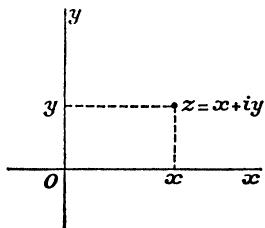
\includegraphics[keepaspectratio]{images/part001_cf49e1ad.jpg}}\\
Figure 7.

The permutation \(z' \to \overline{z}\) of \(\mathbf{C}\) is continuous, and is therefore an automorphism of the topological field \(\mathbf{C}\) .

In fact it is the only automorphism of the topological field C other than the identity automorphism (see Exercise 4).

The functions \(\mathcal{R}(z)\) , \(\mathfrak{J}(z)\) are just the projections of \(\mathbf{R}^2\) onto its factors, and are therefore continuous; the same is true of the absolute value \(|z|\) , since it is the Euclidean norm (Chapter VI, § 2, no. 1) of the point \((x,y)\) in \(\mathbf{R}^2\) .

The properties of the absolute value lead to another proof of the fact that the topology of \(\mathbf{C}\) is compatible with its field structure (cf.~Chapter IX, § 3, no. 2); the continuity of \(z + z'\) follows from the triangle inequality \(|z + z'| \leqslant |z| + |z'|\) ; that of \(zz'\) follows from the relation

\[
\begin{array}{r l} | z z ^ {\prime} - z _ {0} z _ {0} ^ {\prime} | & = | z _ {0} (z ^ {\prime} - z _ {0} ^ {\prime}) + (z - z _ {0}) z _ {0} ^ {\prime} + (z - z _ {0}) (z ^ {\prime} - z _ {0} ^ {\prime}) | \\ & \leqslant | z _ {0} | \cdot | z ^ {\prime} - z _ {0} ^ {\prime} | + | z _ {0} ^ {\prime} | \cdot | z - z _ {0} | + | z - z _ {0} | \cdot | z ^ {\prime} - z _ {0} ^ {\prime} |; \end{array}
\]

lastly, the continuity of \(z^{-1}\) follows from the relation

\[
\left| z _ {0} ^ {- 1} - z ^ {- 1} \right| = | z | ^ {- 1}. \left| z - z _ {0} \right|. \left| z _ {0} \right| ^ {- 1}.
\]

\subsection{THE MULTIPLICATIVE GROUP C*}

We know from Chapter III, § 6, no. 7 that the topology induced on the multiplicative group \(\mathbf{C}^*\) of non-zero complex numbers is compatible with the group structure of \(\mathbf{C}^*\) . Since \(\mathbf{C}^*\) is open in \(\mathbf{C}\) , it follows that \(\mathbf{C}^*\) is a locally compact topological group (Chapter I, § 9, no. 7, Proposition 13) and therefore complete (with respect to the multiplicative uniformity; cf.~Chapter III, § 6, no. 8, Proposition 8). The multiplicative group \(\mathbf{R}_+^*\) of real numbers \(>0\) is a closed subgroup of \(\mathbf{C}^*\) . Another subgroup is the set \(\mathbf{U}\) of complex numbers of absolute value 1, which is identified with the unit circle \(\mathbf{S}_1\) of \(\mathbf{R}^2\) , and is therefore a compact group. Moreover:

PROPOSITION 1. The topological group \(\mathbf{C}^*\) is isomorphic to the product of the topological groups \(\mathbf{R}^*\) and \(\mathbf{U}\) .

For the mapping \(z \to \left( |z|, \frac{z}{|z|} \right)\) is a homeomorphism of \(\mathbf{C}^*\) onto \(\mathbf{R}_+^* \times \mathbf{U}\) (Chapter VI, § 2, no. 3, Proposition 3); and it follows immediately that it is an isomorphism of the group structures.

The topological group \(\mathbf{R}_{+}^{*}\) is already known to be isomorphic to the additive group \(\mathbf{R}\) (Chapter V, § 4, Theorem 1); the study of the topological group \(\mathbf{C}^{*}\) is therefore reduced to that of \(\mathbf{U}\) , which we shall consider in § 2.

\subsection{THE DIVISION RING OF QUATERNIONS}

It follows from Theorem 1 that the field R is a maximal ordered field, and therefore the only non-commutative division ring of finite rank over R is (up to isomorphism) the division ring of quaternions over R; it is denoted by H and is called the division ring of real quaternions (or simply the division ring of quaternions, when there is no fear of confusion). Since H is of rank 4 over the field R, we can define a topology on H homeomorphic to that of \(R^{4}\) (Chapter VI, § 1, no. 5). To be precise, we shall usually identify H with \(R^{4}\) , the elements 1, i, j, k of the canonical basis of H being identified respectively with the vectors \(e_{0}, e_{1}, e_{2}, e_{3}\) of the canonical basis of \(R^{4}\) .

We recall that the multiplication table of the canonical basis of H is given by the formulae

\[
\begin{array}{c} i ^ {2} = j ^ {2} = k ^ {2} = - \mathrm{I}, \quad i j = - j i = k, \\ j k = - k j = i, \quad k i = - i k = j. \end{array}
\]

The topology of H is compatible not only with the ring structure of H (Chapter VI, § 1, no. 5) but also with its division ring structure; for if x is a non-zero quaternion, the coordinates of \(x^{-1}\) are rational functions of those of x, whose denominators do not vanish. The division ring H, endowed with this topology, is therefore a non-commutative topological division ring. The quaternions \(a + bi\) (a, b real) form a (topological) subfield of H, isomorphic to the field C, with which it is often identified.

We have thus a third example of a locally compact, connected topological division ring, the others being R and C. In fact these are the only topological division rings with these two properties.

We know from algebra that the reduced norm of a quaternion \(x = x_{0} + x_{1}i + x_{2}j + x_{3}k\) is

\[
\mathrm{N} (\boldsymbol {x}) = x _ {0} ^ {2} + x _ {1} ^ {2} + x _ {2} ^ {2} + x _ {3} ^ {2} = | | \boldsymbol {x} | | ^ {2}
\]

(it is therefore the square of the Euclidean norm of x). Since

\[
\mathrm{N} (\boldsymbol {x y}) = \mathrm{N} (\boldsymbol {x}) \mathrm{N} (\boldsymbol {y}),
\]

it follows that the set of all quaternions of norm 1, which is identical with the sphere \(S_{3}\) , forms a compact subgroup of the multiplicative group \(H^{*}\) of non-zero quaternions.

PROPOSITION 2. The multiplicative group \(\mathbf{H}^*\) of non-zero quaternions is a topological group isomorphic to the product of its subgroups \(\mathbf{R}_+^*\) and \(\mathbf{S}_3\) .

Every quaternion \(x \neq 0\) can be written as \(x = ||x||.z\) where \(z\) is a quaternion with norm 1; since \(||xx'|| = ||x||.||x'||\) , the mapping \(x \to (||x||, x/||x||)\) of \(H^*\) onto \(R_+^* \times S_3\) is an isomorphism of the group structures, and from Chapter VI, § 2, no. 3, Proposition 3 it is a homeomorphism of \(H^*\) onto \(R_+^* \times S_3\) .

Remarks. 1) With the use of the relations \(||x + y|| \leqslant ||x|| + ||y||\) and \(||xy|| = ||x||.||y||\) it can be proved directly, as with the field of complex numbers in no. 2, that the topology of \(\mathbf{R}^4\) is compatible with the division ring structure of H (cf.~Chapter IX, § 3, no. 2).

\begin{enumerate}
\def\labelenumi{\arabic{enumi})}
\setcounter{enumi}{1}
\item
  From what has been proved it follows that the spheres \(S_{1}\) and \(S_{3}\) can carry a group structure compatible with their topology. We shall see later that, for each integer n other than 1 and 3, there exists no group structure on \(S_{n}\) compatible with the topology of \(S_{n}\) .
\item
  Every point of the group \(\mathbf{S}_3\) has a neighbourhood homeomorphic to \(\mathbf{R}^3\) (Chapter VI, § 2, no. 4, Proposition 5) but \(\mathbf{S}_3\) is not locally isomorphic to \(\mathbf{R}^3\) ; for if it were it would be abelian, since it is connected (Chapter VII, § 2, no. 2, Theorem 1), and this is not the case, since \(i\) and \(j\) belong to \(\mathbf{S}_3\) and \(ij \neq ji\) (cf.~Chapter V, § 3).
\end{enumerate}

\section{ANGULAR MEASURE, TRIGONOMETRIC FUNCTIONS}

\subsection{THE MULTIPLICATIVE GROUP U}

THEOREM 1. The (multiplicative) topological group U of complex numbers of absolute value 1 is isomorphic to the (additive) topological group T of real numbers mod 1.

\(\mathbf{U} = \mathbf{S}_{1}\) is compact and connected, and has a neighbourhood of the identity element \(+1\) homeomorphic to an open interval of \(\mathbf{R}\) (Chapter VI, § 2, no. 4, Proposition 5); the theorem is therefore a consequence of the topological characterization of \(\mathbf{T}\) given in Chapter V, § 3 (Theorem 2).

COROLLARY. The multiplicative group \(\mathbf{C}^*\) of non-zero complex numbers is isomorphic to the group \(\mathbf{R} \times \mathbf{T}\) (cf.~§ 1. no. 3, Proposition 1).

Remark. The isomorphism of the groups \(C^{*}\) and \(R \times T\) implies the existence of roots of every ``binomial equation'' \(z^{n} = a\) in the field C. Using this fact and the local compactness of C we can obtain another proof of the theorem of d'Alembert-Gauss (Exercise 2).

There are only two distinct isomorphisms of the group \(\mathbf{T}\) onto the group \(\mathbf{U}\) ; for if \(g\) , \(g'\) are two isomorphisms of \(\mathbf{T}\) onto \(\mathbf{U}\) , and if \(h'\) is the inverse of \(g'\) , then \(h' \circ g\) is an automorphism of \(\mathbf{T}\) , and therefore (Chapter VII, § 2, no. 4, Proposition 6) we have identically either \(g'(x) = g(x)\) or \(g'(x) = g(-x)\) . We may always assume that \(g\) is such that \(i\) is the image under \(g\) of the class mod \(1\) of the point \(\frac{1}{4}\) ; then, if \(\varphi\) denotes the canonical homomorphism of \(\mathbf{R}\) onto \(\mathbf{T}\) , every strict morphism of the additive group \(\mathbf{R}\) onto the multiplicative group \(\mathbf{U}\) is of the form \(x \to g(\varphi(x/a))\) , where \(a\) is a real number \(\neq o\) (Chapter VII, § 2, no. 3, Proposition 4); note that the interval \([- \frac{1}{2} |a|, \frac{1}{2} |a|]\) is the largest symmetric open interval of \(\mathbf{R}\) which is mapped one-to-one onto its image by this strict morphism, and that we have \(g(\varphi(\frac{1}{4})) = i\) . We shall denote the homomorphism \(x \to g(\varphi(x))\) by \(x \to e(x)\) ; every strict morphism of \(\mathbf{R}\) onto \(\mathbf{U}\) is therefore of the form \(x \to e(x/a)\) , where \(a \neq 0\) . The function \(e(x)\) is continuous on \(\mathbf{R}\) , complex valued, and satisfies the identities

\begin{enumerate}
\def\labelenumi{(\arabic{enumi})}
\tightlist
\item
\end{enumerate}

\[
\left| e (x) \right| = 1,\tag{2}
\]

\[
\boldsymbol {e} (x + y) = \boldsymbol {e} (x) \boldsymbol {e} (y),
\]

together with the relations

\[
e (0) = \mathrm{I}, \quad e (\frac {1}{4}) = i, \quad e (\frac {1}{2}) = - \mathrm{I}, \quad e (\frac {3}{4}) = - i, \quad e (\mathrm{I}) = \mathrm{I}. \tag {3}
\]

From (1) and (2) it follows that

\[
e (- x) = \frac {1}{e (x)} = \overline {{{{e (x)}}}},\tag{4}
\]

and from (2) and (3) that

\[
\begin{array}{l} e (x + \frac {1}{4}) = i e (x), \quad e (x + \frac {1}{2}) = - e (x), \\ e (x + \frac {3}{4}) = - i e (x), \quad e (x + 1) = e (x). \end{array}
\]

Thus the function \(e(x)\) is periodic and has 1 as a principal period.

Remark. The mapping \(x + iy \to e^x e(y)\) is a strict morphism of the additive group \(\mathbf{C}\) onto the multiplicative group \(\mathbf{C}^*\) , and its restriction to a suitable neighbourhood of \(\mathbf{o}\) is a local isomorphism of \(\mathbf{C}\) with \(\mathbf{C}^*\) . Consequently (Chapter VII, § 2, no. 3) every strict morphism of \(\mathbf{C}\) onto \(\mathbf{C}^*\) is of the form \(x + iy \to e^{\alpha x + \beta y} e(\gamma x + \delta y)\) , where \(\alpha, \beta, \gamma, \delta\) are any real numbers such that \(\alpha \delta - \beta \gamma \neq \mathbf{o}\) . We shall see later that there is just one of these homomorphisms, denoted by \(z \rightarrow e^{z}\) , such that

\[
\lim _ {z \rightarrow 0} \frac {e ^ {z} - 1}{z} = 1;
\]

and the restriction of this homomorphism to the real axis is the same as \(e^{x}\) (whence the notation).

\subsection{ANGLES}

Since the field \(\mathbf{R}\) is ordered, we may orient the real number plane \(\mathbf{R}^2\) by taking \(e_1 \wedge e_2\) as positive bivector ( \(e_1, e_2\) being the vectors of the canonical basis). In the oriented real number plane \(\mathbf{R}^2\) (identified with \(\mathbf{C}\) in what follows) we can then define the angle \((\widehat{\Delta_1, \Delta_2})\) of an arbitrary pair of rays ( \(\Delta_1, \Delta_2\) ) with origin \(o\) (*). The set \(\mathfrak{A}\) of all angles has the structure of an abelian group (written additively) defined by

\[
(\widehat {\Delta_ {1} , \Delta_ {3}}) = (\widehat {\Delta_ {1} , \Delta_ {2}}) + (\widehat {\Delta_ {2} , \Delta_ {3}}),
\]

so that, in particular, \((\widehat{\Delta_1, \Delta_1}) = 0\) and \((\widehat{\Delta_2, \Delta_1}) = -(\widehat{\Delta_1, \Delta_2})\) .

The flat angle \(\varpi\) is the solution \(\neq 0\) of the equation \(2\theta = 0\) in \(\mathfrak{A}\) ; it is the angle which the negative real semi-axis makes with the positive real semi-axis.

If z is any non-zero complex number, the amplitude (or argument) of z, denoted by \(\operatorname{Am}(z)\) , is the angle which the ray through z with origin o makes with the positive real semi-axis. The mapping \(z \to \operatorname{Am}(z)\) is a homomorphism of the multiplicative group \(C^{*}\) onto the additive group A, and therefore we have

\[
\operatorname{Am} \left(z z ^ {\prime}\right) = \operatorname{Am} (z) + \operatorname{Am} \left(z ^ {\prime}\right) \quad \text { and } \quad \operatorname{Am} (\bar {z}) = \operatorname{Am} \left(z ^ {- 1}\right) = - \operatorname{Am} (z).
\]

The angle \(\delta = \operatorname{Am}(i)\) is called the positive right angle; it is one of the solutions in A of the equation \(2\theta = \varpi\) , the other one being \(-\delta = \delta + \varpi\) .

The homomorphism \(z \to \operatorname{Am}(z)\) , restricted to the subgroup \(\mathbf{U}\) of \(\mathbf{C}^*\) , is an isomorphism of the group structure of \(\mathbf{U}\) onto that of \(\mathfrak{A}^{(**)}\) ; if we use this isomorphism to transport the topology of U to the group A, the latter group becomes a compact topological group, and the mapping \(z \to \operatorname{Am}(z)\) of \(C^{*}\) onto A is a strict morphism of the topological group \(C^{*}\) onto the topological group A.

Let us denote by \(\theta \to f(\theta)\) the isomorphism of \(\mathfrak{A}\) onto \(\mathbf{U}\) which is the inverse of the isomorphism \(z \to \operatorname{Am}(z)\) of \(\mathbf{U}\) onto \(\mathfrak{A}\) . By definition \(\mathcal{R}(f(\theta))\) is denoted by \(\cos \theta\) and is called the cosine of the angle \(\theta\) ; \(\mathfrak{J}(f(\theta))\) is denoted by \(\sin \theta\) and is called the sine of the angle \(\theta\) . These functions are continuous on the topological group \(\mathfrak{A}\) , and satisfy the following relations (loc. cit.), which are immediate consequences of the definitions above:

\[
\begin{array}{r l} \cos o = 1, & \sin o = 0, \quad \cos \varpi = - 1, \quad \sin \varpi = 0, \\ \cos (- \theta) = \cos \theta , & \sin (- \theta) = - \sin \theta , \\ \cos (\theta + \theta^ {\prime}) = \cos \theta \cos \theta^ {\prime} - \sin \theta \sin \theta^ {\prime}, \\ \sin (\theta + \theta^ {\prime}) = \sin \theta \cos \theta^ {\prime} + \sin \theta^ {\prime} \cos \theta , \\ \cos^ {2} \theta + \sin^ {2} \theta = 1. \end{array}
\]

By definition, the tangent of an angle \(\theta \in \mathfrak{A}\) is defined, whenever \(\cos \theta \neq 0\) , to be \(\sin \theta / \cos \theta\) (loc. cit.) and is denoted by \(\tan \theta\) ; it is a continuous function, which extends by continuity to \(\tilde{\mathbf{R}}\) (Chapter VI, § 3, no. 4) by taking the value \(\infty\) for the angles \(\delta\) and \(-\delta\) . We have \(\tan (\theta + \varpi) = \tan \theta\) . The cotangent of \(\theta\) , denoted by \(\cot \theta\) , is the element of \(\tilde{\mathbf{R}}\) equal to \(1 / \tan \theta\) .

Note that, if \(\operatorname{Am}(z) = \theta\) , we have \(z = |z| (\cos \theta + i \sin \theta)\) ; this expression is called the trigonometric form of the complex number \(z \neq 0\) .

\subsection{ANGULAR MEASURE}

By Theorem 1 of no. 1, the topological group \(\mathfrak{A}\) of angles is isomorphic to \(\mathbf{T}\) . Every strict morphism of \(\mathbf{R}\) onto \(\mathfrak{A}\) can be obtained by composing the isomorphism \(z \to \operatorname{Am}(z)\) of \(\mathbf{U}\) onto \(\mathfrak{A}\) with a strict morphism of \(\mathbf{R}\) onto \(\mathbf{U}\) ; if we put \(\Im(x) = \operatorname{Am}(e(x))\) , every strict morphism of \(\mathbf{R}\) onto \(\mathfrak{A}\) is therefore of the form \(x \to \Im(x/a)\) ( \(a \neq 0\) ). Given a real number \(a > 0\) , fixed once and for all, every angle \(\theta\) corresponds, by the homomorphism \(x \to \Im(x/a)\) , to a class of real numbers mod \(a\) (i.e., an element of \(\mathbf{Z}/a\mathbf{Z}\) ) which is called the measure of \(\theta\) relative to the base \(a\) ; by abuse of language, every real number in this class is also called a measure of \(\theta\) ; the angle \(\Im(x/a)\) is called the angle with measure \(x\) (relative to the base a). If x is a measure of \(\theta\) and \(x'\) a measure of \(\theta'\) (relative to the same base) then \(x + x'\) is a measure of \(\theta + \theta'\) , and -x is a measure of - \(\theta\) . The principal measure of an angle (relative to the base a) is that one of its measures which lies in the interval {[}0, a{]}.

Choice of a base \(a\) . We restrict ourselves always to bases \(a > 1\) . To each \(a > 1\) corresponds an angle \(\omega = \Im(1/a)\) whose principal measure is \(1\) , and which is called the unit of angular measure relative to the base \(a\) ; conversely, to each angle \(\omega \neq 0\) there corresponds a unique \(a > 1\) such that \(\Im(1/a) = \omega\) , so that knowledge of the unit of angular measure determines the base \(a > 1\) entirely.

In numerical calculations one usually takes either \(a = 360\) or \(a = 400\) ; the corresponding unit of angular measure is called the degree ( \(a = 360\) ) or the grade ( \(a = 400\) ).

In analysis, and indeed in all branches of mathematics where numerical calculation is not involved, the base a defined by the condition

\[
\lim _ {x \rightarrow 0} \frac {e (x / a) - 1}{x} = 1
\]

is universally used; this base is denoted by \(2\pi\) . The corresponding unit of angular measure is called a radian, and the measure is called radian measure; with the definition of \(e^{z}\) for complex z mentioned earlier, we have \(\boldsymbol{e}(x)=e^{2\pi ix}\) for all \(x\in R\) .

Once the base a has been chosen, when one speaks of an angle one usually means a measure of this angle relative to the base a; this abuse of language has no drawback provided (as is always the case when numerical calculations are not involved) the base a remains fixed throughout, and provided that one remembers that two real numbers which are congruent mod a correspond to the same angle.

For example, what is usually understood by the amplitude of a complex number \(z \neq 0\) is a radian measure of this angle, determined by conventions which will depend on the question under consideration; once these conventions have been made, the measure of the amplitude thus chosen is denoted by Am (z).

\subsection{TRIGONOMETRIC FUNCTIONS}

If we compose the functions \(\cos\theta\) , \(\sin\theta\) , \(\tan\theta\) , \(\cot\theta\) (defined on A) with the homomorphism \(x\to\Im(x/a)\) of R onto A, the functions

\[
\cos \Im \left(\frac {x}{a}\right), \quad \sin \Im \left(\frac {x}{a}\right), \quad \tan \Im \left(\frac {x}{a}\right), \quad \cot \Im \left(\frac {x}{a}\right)
\]

so obtained are called respectively the cosine, sine, tangent and cotangent of the number \(x\) relative to the base \(a\) , and are written \(\cos_a x\) , \(\sin_a x\) , \(\tan_a x\) , \(\cot_a x\) . The mapping \(x \to \cos_a x + i \sin_a x\) is the composition of \(\theta \to \cos \theta + i \sin \theta\) and \(x \to \Im(x/a)\) , so that, from the definition of \(\cos \theta\) and \(\sin \theta\) in no. 2, we have the identity

\[
e \left(\frac {x}{a}\right) = \cos_ {a} x + i \sin_ {a} x,\tag{5}
\]

which is equivalent to

\[
\cos_ {a} x = \Re \left(e \left(\frac {x}{a}\right)\right), \quad \sin_ {a} x = \Im \left(e \left(\frac {x}{a}\right)\right),
\]

and also, by (4), equivalent to

\[
\cos_ {a} x = \frac {\mathrm{I}}{2} \left(e \left(\frac {x}{a}\right) + e \left(- \frac {x}{a}\right)\right), \quad \sin_ {a} x = \frac {\mathrm{I}}{2 i} \left(e \left(\frac {x}{a}\right) - e \left(- \frac {x}{a}\right)\right).
\]

Hence the identities

\[
\cos_ {b} x = \cos_ {a} \left(\frac {a x}{b}\right), \quad \sin_ {b} x = \sin_ {a} \left(\frac {a x}{b}\right).\tag{6}
\]

The only trigonometric functions which arise in branches of mathematics where numerical calculation is not involved are those relative to the base \(2\pi\) referred to above; these functions are denoted simply by \(\cos x\) , \(\sin x\) , \(\tan x\) , \(\cot x\) in place of \(\cos_{2\pi}x\) , \(\sin_{2\pi}x\) , \(\tan_{2\pi}x\) , \(\cot_{2\pi}x\) . For the purposes of numerical calculation, there are tables of the trigonometric functions corresponding to the bases a = 360 and a = 400; and the formulae (6) allow us to deduce the values of the trigonometric functions relative to any other base.

The relations recalled earlier between the cosines and sines of angles evidently give rise to the same relations between the cosines and the sines of the numbers which measure these angles; in particular, we have

\[
\begin{array}{r l} & {\cos_ {a} (x + y) = \cos_ {a} x \cos_ {a} y - \sin_ {a} x \sin_ {a} y,} \\ & {\sin_ {a} (x + y) = \sin_ {a} x \cos_ {a} y + \sin_ {a} y \cos_ {a} x,} \\ & {\cos_ {a} (- x) = \cos_ {a} x, \qquad \sin_ {a} (- x) = - \sin_ {a} x,} \\ & {\qquad \cos_ {a} ^ {2} x + \sin_ {a} ^ {2} x = 1.} \end{array}
\]

The functions \(\cos_{a}x\) and \(\sin_{a}x\) are continuous on R, and are periodic with period a; moreover, a is a principal period of these functions, for the relation \(\cos_{a}x = \cos_{a}y\) implies that either \(\sin_{a}x = \sin_{a}y\) or

\[
\sin_ {a} x = - \sin_ {a} y, \quad \text { i.e., }
\]

\[
e \left(\frac {x}{a}\right) = e \left(\frac {y}{a}\right) \quad \text { or } \quad e \left(\frac {x}{a}\right) = e \left(- \frac {y}{a}\right),
\]

so that either

\[
x \equiv y (\mathrm{mod} a) \quad \text { or } \quad x \equiv - y (\mathrm{mod} a);
\]

and similarly

\[
\sin_ {a} x = \sin_ {a} y
\]

is equivalent to either \(x \equiv y \pmod{a}\) or \(x + y \equiv \frac{1}{2} a \pmod{a}\) .

It follows from this that \(\cos_{a}x\) never takes the same value twice in the interval \([0,\frac{1}{2}a]\) ; hence, when restricted to this interval, it is a bijective mapping of this interval onto the interval \([-1,+1]\) . Since \(\cos_{a}0=1\) and \(\cos_{a}\left(\frac{1}{2}a\right)=-1\) , \(x\to\cos_{a}x\) is a strictly decreasing mapping of \([0,\frac{1}{2}a]\) onto \([-1,1]\) (Chapter IV, § 2, no. 6, Theorem 5 and Remark). We have \(\cos_{a}x=0\) for x=a/4, \(\cos_{a}x>0\) for \(0\leqslant x<a/4\) , \(\cos_{a}x<0\) for \(a/4<x\leqslant a/2\) . Since \(\cos_{a}(-x)=\cos_{a}x\) we can deduce how \(\cos_{a}x\) varies in the interval \([-\frac{1}{2}a,0]\) , and hence throughout the whole of R by periodicity (Fig. 8). Since \(\sin_{a}x=-\cos_{a}(x+a/4)\) we can also deduce how \(\sin_{a}x\) varies in R (Fig. 8).

\pandocbounded{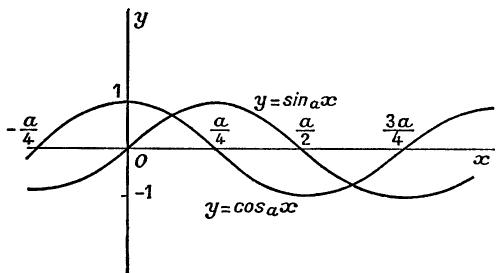
\includegraphics[keepaspectratio]{images/part001_7529c0a8.jpg}}\\
Figure 8.

The function \(\tan_{a}x\) is a continuous mapping of \(\mathbf{R}\) onto \(\tilde{\mathbf{R}}\) ; it takes the value \(\infty\) for the values \(\frac{1}{4} a + \frac{1}{2} ka\) ( \(k \in \mathbf{Z}\) ). Since \(\frac{1}{2} a\) is a period of \(\tan_{a}x\) , it is a principal period. In the interval \([0, \frac{1}{4} a]\) , \(\sin_{a}x\) increases from \(0\) to \(1\) , \(\cos_{a}x\) decreases from \(1\) to \(0\) , and therefore \(\tan_{a}x\) is strictly increasing in \([0, \frac{1}{4} a[\) and maps this interval onto \([0, +\infty[\) ; it follows that \(\tan_{a}x\) is strictly increasing in the interval \(]-\frac{1}{4}a,+\frac{1}{4}a[.\) and is a homeomorphism of this interval onto R (Fig. 9).

\pandocbounded{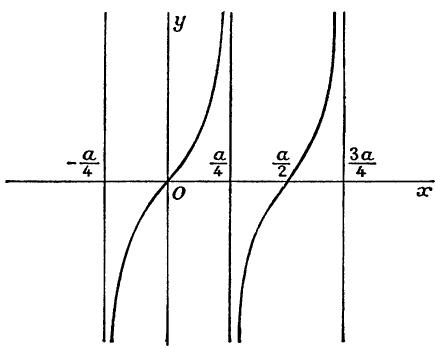
\includegraphics[keepaspectratio]{images/part001_329f289a.jpg}}\\
Figure 9.

\subsection{ANGULAR SECTORS}

Given two distinct closed rays \(\Delta_{1}, \Delta_{2}\) with origin \(o\) , let \(x\) be the principal measure of the angle \((\widehat{\Delta_{1}, \Delta_{2}})\) (relative to a base \(a\) , chosen once and for all). The union of the closed (resp. open) rays \(\Delta\) with origin \(o\) which are such that the principal measure \(y\) of the angle \((\widehat{\Delta_{1}, \Delta})\) satisfies \(o \leqslant y \leqslant x\) (resp. \(o < y < x\) ) is the closed (resp. open) angular sector \(S\) with origin \(\Delta_{1}\) and extremity \(\Delta_{2}\) , as defined in algebra. For by means of a rotation we can always reduce to the case where \(S\) does not contain the ray through the point \(-1\) . If \(\alpha\) and \(\beta\) are then the angles which \(\Delta_{1}\) and \(\Delta_{2}\) respectively make with the positive real semi-axis, then the closed angular sector \(S\) is the union of the closed half-lines \(\Delta\) which make an angle \(\theta\) with the positive real semi-axis such that \(\tan \frac{1}{2} \alpha \leqslant \tan \frac{1}{2} \theta \leqslant \tan \frac{1}{2} \beta\) . Now if \(u, v, t\) are the measures of \(\alpha, \beta, \theta\) respectively which lie in the interval \([- \frac{1}{2} a, + \frac{1}{2} a[\) , these inequalities are equivalent to \(\tan_{a} \frac{1}{2} u \leqslant \tan_{a} \frac{1}{2} t \leqslant \tan_{a} \frac{1}{2} v\) ; and since \(\tan_{a} x\) is an increasing function in the interval \([- \frac{1}{4} a, + \frac{1}{4} a[\) , they are also equivalent to \(u \leqslant t \leqslant v\) , or to \(o \leqslant t - u \leqslant v - u\) ; since \(x = v - u\) , \(y = t - u\) , the result is proved for closed angular sectors, and the proof for open ones is similar.

A closed angular sector is a closed set in \(R^{2}\) , and the open angular sector with the same origin and the same extremity is its interior in \(R^{2}\) (Chapter VI, § 2, no. 3, Proposition 3). The angle \((\widehat{\Delta_1, \Delta_2})\) , with principal measure \(x\) , is called the angle of the sector S; S is said to be salient if \(x < \frac{1}{2} a\) , flat (or a closed half-plane) if \(x = \frac{1}{2} a\) ; re-entrant if \(x > \frac{1}{2} a\) . A salient angular sector is acute if \(x < \frac{1}{4} a\) , right if \(x = \frac{1}{4} a\) , obtuse if \(x > \frac{1}{4} a\) . The bisector of the sector S is the ray \(\Delta\) which makes an angle \(y = \frac{1}{2} x\) with \(\Delta_1\) .

\pandocbounded{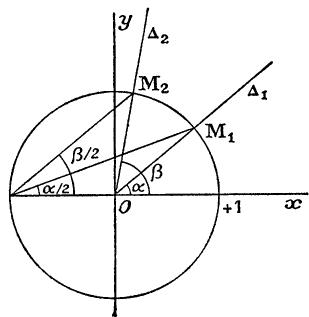
\includegraphics[keepaspectratio]{images/part001_1c4c55ab.jpg}}\\
Figure 10.

Two distinct closed rays \(\Delta_{1}, \Delta_{2}\) determine two closed angular sectors; their union is the real plane \(R^{2}\) , and their intersection is \(\Delta_{1} \cup \Delta_{2}\) .

\subsection{CROSSES}

We have also defined in algebra the cross of a pair of lines in a two-dimensional vector space over a maximal ordered field (*). This definition applies in particular to the real plane \(\mathbf{R}^2\) . The set \(\mathfrak{A}_0\) of all crosses has the structure of an abelian group (written additively) defined by

\[
(\widehat {\mathbf {D _ {1} , D _ {3}}}) = (\widehat {\mathbf {D _ {1} , D _ {2}}}) + (\widehat {\mathbf {D _ {2} , D _ {3}}})
\]

so that, in particular, \((\widehat{\mathbf{D}_1,\mathbf{D}_1}) = 0\) and \((\widehat{\mathbf{D}_2,\mathbf{D}_1}) = -(\widehat{\mathbf{D}_1,\mathbf{D}_2}).\)

The right cross \(\delta_0\) is the solution \(\neq 0\) of the equation \(2\theta = 0\) in \(\mathfrak{A}_0\) ; it is the cross which the imaginary axis makes with the real axis.

We define a canonical homomorphism \(\varphi\) of the group \(\mathfrak{A}\) of angles onto the group \(\mathfrak{A}_0\) of crosses by making correspond to the angle which a ray \(\Delta\) makes with the positive real semi-axis, the cross which the line D containing \(\Delta\) makes with the real axis. A cross \(\theta_0\) is the image under \(\varphi\) of two angles \(\theta\) and \(\theta + \varpi\) ; thus \(\mathfrak{A}_0\) is isomorphic to the quotient of \(\mathfrak{A}\) by the subgroup \(\{o, \varpi\}\) . If we transport to \(\mathfrak{A}_0\) the topology of the quotient group \(\mathfrak{A}/\{o, \varpi\}\) by means of the bijective homomorphism associated with \(\varphi\) , then \(\mathfrak{A}_0\) becomes a compact topological group and \(\varphi\) a strict morphism of \(\mathfrak{A}\) onto \(\mathfrak{A}_0\) .

If we compose the homomorphism \(\varphi\) of \(\mathfrak{A}\) onto \(\mathfrak{A}_0\) with the homomorphism \(x \to \Im(x/a)\) of \(\mathbf{R}\) onto \(\mathfrak{A}\) , we have a homomorphism \(x \to \Im_0(x/a)\) of \(\mathbf{R}\) onto \(\mathfrak{A}_0\) ; every cross \(\theta_0 \in \mathfrak{A}_0\) corresponds, under this homomorphism, to a class of real numbers mod \(\frac{1}{2}a\) , which is called the measure of the cross \(\theta_0\) (relative to the base \(a\) ); by abuse of language, every number in this class is called a measure of \(\theta_0\) , and that one which belongs to the interval \([0, \frac{1}{2}a]\) is called the principal measure of \(\theta_0\) ; the cross \(\Im_0(x/a)\) is the cross of measure \(x\) . Every measure of \(\theta_0\) is also a measure of one of the two angles \(\theta, \theta + \varpi\) whose image under the homomorphism \(\varphi\) is \(\theta_0\) .

Here again, once the base a has been chosen, when we speak of a cross we generally mean, by abuse of language, a measure of this cross relative to the base a.

Remark. We can define a homomorphism of \(\mathbf{C}^*\) onto \(\mathfrak{A}_0\) by mapping each complex number \(z \neq 0\) to the cross which the line through \(0\) and \(z\) makes with the real axis. Clearly this homomorphism is the composition of \(\varphi\) and the homomorphism \(z \to \operatorname{Am}(z)\) of \(\mathbf{C}^*\) onto \(\mathfrak{A}\) ; it is therefore a strict morphism of the topological group \(\mathbf{C}^*\) onto the topological group \(\mathfrak{A}_0\) , and the associated bijective homomorphism is an isomorphism of the quotient group \(\mathbf{C}^*/\mathbf{R}^*\) onto \(\mathfrak{A}_0\) .

We know that if D denotes a line making a cross \(\theta_0\) with the real axis and if \((a, b)\) is a pair of direction ratios of D, then the tangent of the cross \(\theta_0\) (denoted by tan \(\theta_0\) ) is the element \(b/a\) of \(\tilde{\mathbf{R}} (= \infty\) if \(a = 0\) ), which is also called the slope of the line D. If \(\theta\) and \(\theta + \varpi\) are the two angles whose image under \(\varphi\) is \(\theta_0\) , then we have \(\tan \theta_0 = \tan \theta = \tan (\theta + \varpi)\) . The mapping \(\theta_0 \to \tan \theta_0\) is a homeomorphism of \(\mathfrak{A}_0\) onto \(\tilde{\mathbf{R}}\) , for the topological space \(\mathbf{C}^*/\mathbf{R}^*\) is just the real projective line \(\mathbf{P}_1\) , and from Chapter VI, § 3, no. 3, the mapping of a line (considered as a point of \(\mathbf{P}_1\) ) to its slope is a homeomorphism of \(\mathbf{P}_1\) onto \(\tilde{\mathbf{R}}\) . If now we transport to \(\tilde{\mathbf{R}}\) the group structure of \(\mathfrak{A}_0\) by means of the mapping \(\theta_0 \to \tan \theta_0\) , we have defined on \(\tilde{\mathbf{R}}\) the structure of an abelian topological group, in which the product of two elements \(t_1\) , \(t_2\) is \(\frac{t_1 + t_2}{1 - t_1 t_2}\) whenever \(t_1\) , \(t_2\) belong to R and \(t_1 t_2 \neq 1\) ; for pairs \((t_1, t_2)\) which do not satisfy these conditions, the product of \(t_{1}\) and \(t_{2}\) is obtained by extending the function \(\frac{x+y}{1-xy}\) by continuity to \(\tilde{R}\times\tilde{R}\) , and is still denoted by \(\frac{t_{1}+t_{2}}{1-t_{1}t_{2}}\) .

\section{INFINITE SUMS AND PRODUCTS OF COMPLEX NUMBERS}

\subsection{INFINITE SUMS OF COMPLEX NUMBERS}

Since the additive group of the field C is the same as the additive group \(R^{2}\) , it is not necessary to make a special study of summable families and series in C, since this is included in the general theory of Chapter VII, § 3; we leave to the reader the exercise of translating the results of this theory into the language of the theory of complex numbers. We state only the following proposition, which is a corollary to Proposition 3 of Chapter VII, § 3, no. 1:

PROPOSITION 1. If \((u_{\lambda})_{\lambda \in \mathbf{L}}\) and \((v_{\mu})_{\mu \in \mathbf{M}}\) are two summable families of complex numbers, then the family \((u_{\lambda}v_{\mu})_{(\lambda ,\mu)\in \mathbf{L}\times \mathbf{M}}\) is summable and we have

\[
\sum_ {(\lambda , \mu) \in \mathbf {L} \times \mathbf {M}} u _ {\lambda} v _ {\mu} = \left(\sum_ {\lambda \in \mathbf {L}} u _ {\lambda}\right) \left(\sum_ {\mu \in \mathbf {M}} v _ {\mu}\right).\tag{1}
\]

We leave it to the reader to state the corresponding result for quaternions.

\subsection{MULTIPLIABLE FAMILIES IN C*}

In the multiplicative group \(\mathbf{C}^*\) of non-zero complex numbers a family \((z_{i})_{i\in I}\) cannot be multipliable unless \(\lim z_{i} = 1\) with respect to the filter of complements of finite subsets of \(I\) (Chapter III, § 5, no. 2, Proposition 1); furthermore, since every point of \(\mathbf{C}^*\) has a countable fundamental system of neighbourhoods, the set of indices \(i\) such that \(z_{i}\neq 1\) is countable if the family \((z_{i})\) is multipliable (Chapter III, § 5, no. 2, Corollary to Proposition 1).

PROPOSITION 2. A family \((z_{t})\) of complex numbers \(z_{t} = r_{t}(\cos \theta_{t} + i\sin \theta_{t})\) is multipliable if and only if the family \((r_{t})\) of absolute values of the \(z_{t}\) is multipliable in \(\mathbf{R}_{+}^{*}\) and the family \((\theta_{t})\) of amplitudes of the \(z_{t}\) is summable in the group of angles \(\mathfrak{A}\) .

In view of the structure of the group \(\mathbf{C}^*\) ( \(\S\) 1, no. 3, Proposition 1), the proposition is an immediate consequence of Proposition 4 of Chapter III, \(\S\) 5, no. 4.

If we map each angle \(\theta\) to that one of its measures (to any given base \(a\) ) which belongs to the interval \([- \frac{1}{2} a, \frac{1}{2} a]\) , we have a local isomorphism of \(\mathfrak{A}\) with \(\mathbf{R}\) ( \(\S 2\) , no. 2); since \(\lim \theta_{t} = 0\) with respect to the filter of complements of finite subsets of \(\mathbf{I}\) , we may replace the condition (in the statement of Proposition 2) that the family \(\theta_t\) should be summable in \(\mathfrak{A}\) by the condition that the family \((t_t)\) of measures of the angles \(\theta_t\) which belong to \([- \frac{1}{2} a, \frac{1}{2} a]\) should be summable in \(\mathbf{R}\) .

The following theorem gives another criterion for a family of complex numbers, put in the form \((\mathbf{1} + u_{\iota})\) , to be multipliable in \(\mathbf{C}^*\) . (It generalizes Theorem 4 of Chapter IV, § 7, no. 4; see also Chapter IX, Appendix, no. 2, Proposition 1):

THEOREM 1. The family \((\mathbf{1} + u_{\iota})_{\iota \in \mathbf{I}}\) is multipliable in \(\mathbf{C}^*\) if and only if the family \((|u_{\iota}|)\) is summable in \(\mathbf{R}\) .

For each finite subset J of I, put

\[
p _ {J} = \prod_ {\iota \in J} (\mathbf{1} + a _ {\iota}), \quad s _ {J} = \sum_ {\iota \in J} a _ {\iota}, \quad \sigma_ {J} = \sum_ {\iota \in J} | a _ {\iota} |.
\]

LEMMA 1. For each finite subset J of I, let \(\varphi(J) = \sup_{L \subset J} (p_L - 1)\) . Then for each subset L of J we have

\[
\left| p _ {\mathbf {L}} - \mathbf {1} - s _ {\mathbf {L}} \right| \leqslant \varphi (\mathrm{J}) \sigma_ {\mathbf {L}}.\tag{2}
\]

This is clear if L is empty. We proceed by induction on card (L). Let \(L = K \cup \{\lambda\}\) , where \(\lambda \notin K\) ; then \(p_{\mathbf{L}} = p_{\mathbf{K}}(\mathbf{1} + a_{\lambda})\) and \(s_{\mathbf{L}} = s_{\mathbf{K}} + a_{\lambda}\), so that \(p_{\mathbf{L}} - \mathbf{1} - s_{\mathbf{L}} = (p_{\mathbf{K}} - \mathbf{1} - s_{\mathbf{K}}) + (p_{\mathbf{K}} - \mathbf{1})a_{\lambda}\) ; hence, by the inductive hypothesis and the definition of \(\varphi(\mathbf{J})\) , we have

\[
\left| p _ {\mathrm{L}} - \mathrm{1} - s _ {\mathrm{L}} \right| \leqslant \varphi (\mathrm{J}) \sigma_ {\mathrm{K}} + \varphi (\mathrm{J}) \left| a _ {\lambda} \right| = \varphi (\mathrm{J}) \sigma_ {\mathrm{L}},
\]

which proves the lemma.

LEMMA 2. If J is a finite subset of I such that \(\varphi(J) < 1/4\) , then

\[
\left| \sigma_ {J} \right| \leqslant 4 \varphi (J) / (1 - 4 \varphi (J)).
\]

For since \(\sigma_{\mathbf{L}} \leqslant \sigma_{\mathbf{J}}\) for all subsets \(\mathbf{L}\) of \(\mathbf{J}\) , it follows from (2) that \(|s_{\mathbf{L}}| \leqslant \varphi(\mathbf{J})\sigma_{\mathbf{J}} + |p_{\mathbf{L}} - \mathbf{1}| \leqslant (\mathbf{1} + \sigma_{\mathbf{J}})\varphi(\mathbf{J})\) ; but by virtue of Chapter VII, §3, no. 1, Proposition 2, we have \(|\sigma_{\mathbf{J}}| \leqslant 4\sup_{\mathbf{L} \subset \mathbf{J}} |s_{\mathbf{L}}|\) , hence \(\sigma_{\mathbf{J}} \leqslant 4\varphi(\mathbf{J})(\mathbf{1} + \sigma_{\mathbf{J}})\) , and the result follows.

Now let us show that the condition stated in Theorem 1 is sufficient. The hypothesis that the family \((|u_{\iota}|)\) is summable in \(\mathbf{R}\) implies that the family \((\mathrm{1} + |u_{\iota}|)\) is multipliable in \(\mathbf{R}_{+}^{*}\) (Chapter IV, § 7, no. 4, Theorem 4); hence, for each \(\varepsilon > 0\) , there is a finite subset \(J_{0}\) of I such that, for each finite subset L of I which does not meet \(J_{0}\) , we have \(\prod_{\iota \in L} (\mathrm{1} + |u_{\iota}|) - \mathrm{1} \leqslant \varepsilon\) . But we can write \(\prod_{\iota \in L} (\mathrm{1} + u_{\iota}) - \mathrm{1}\) in the form \(\sum_{M} \left( \prod_{\iota \in M} u_{\iota} \right)\) where M runs through all non-empty subsets of L; and since \(\left| \prod_{\iota \in M} u_{\iota} \right| = \prod_{\iota \in M} |u_{\iota}|\) , we have

\[
\left| \prod_ {\iota \in L} (1 + u _ {\iota}) - 1 \right| \leqslant \sum_ {M} \left(\prod_ {\iota \in M} | u _ {\iota} |\right) = \prod_ {\iota \in L} (1 + | u _ {\iota} |) - 1 \leqslant \varepsilon .
\]

This proves our assertion, by virtue of Cauchy's criterion, since \(\mathbf{C}^*\) is a complete group.

We still have to show that the condition of Theorem 1 is necessary. If \((\mathbf{1} + u_{\iota})_{\iota\in \mathbf{I}}\) is a multipliable family in \(\mathbf{C}^*\) , there exists a finite subset \(J\) of \(I\) such that, for every finite subset \(H\) of \(I\) which does not meet \(J\) , we have \(\left|\prod_{\iota\in H}(1 + u_{\iota}) - 1\right| \leqslant 1/8\) . By Lemma 2, it follows that \(\sum_{\iota\in H}|u_{\iota}| \leqslant 1\) for every finite subset \(H\) of \(I\) which does not meet \(J\) , and hence the family \((|u_{\iota}|)\) is summable in \(\mathbf{R}\) (Chapter IV, § 7, no. 1, Theorem 1).

The proof above applies also, mutatis mutandis, to (ordered) infinite products in certain non-commutative division rings and algebras (see Exercise 6, and Chapter IX, Appendix).

\subsection{INFINITE PRODUCTS OF COMPLEX NUMBERS}

For an infinite product of non-zero complex numbers with general factor \(z_{n} = r_{n}(\cos \theta_{n} + i\sin \theta_{n})\) to be convergent in \(\mathbf{C}^{*}\) , it is necessary and sufficient, from the structure of the group \(\mathbf{C}^{*}\) , that the product with general factor \(r_{n}\) converge in \(\mathbf{R}_{+}^{*}\) and the series with general term \(t_{n}\) (the measure of \(\theta_{n}\) which lies in \(] - \frac{1}{2} a, \frac{1}{2} a]\) ) converge in \(\mathbf{R}\) .

DEFINITION 1. An infinite product of complex numbers, with general factor \(1 + u_{n}\) , is said to be absolutely convergent if the product with general factor \(1 + |u_{n}|\) is convergent (or, equivalently, if the series with general term \(|u_{n}|\) is convergent).

PROPOSITION 3. An infinite product of complex numbers is commutatively convergent if and only if it is absolutely convergent.

This follows from Proposition 9 of Chapter III, § 5, no. 7, and Theorem 1 of no. 2 above.

Remarks. 1) The product with general factor \(|1 + u_n|\) can be convergent, and indeed absolutely convergent in \(\mathbf{R}_+^*\) , without the convergence of the product with general factor \(1 + |u_n|\) (see Exercise 4); of course, this cannot happen if all the \(u_n\) are real and \(>0\) from a certain index onwards.

\begin{enumerate}
\def\labelenumi{\arabic{enumi})}
\setcounter{enumi}{1}
\tightlist
\item
  As already remarked for products of factors \textgreater0, the convergence of the series with general term \(u_{n}\) is neither necessary nor sufficient for the convergence of the product with general factor \(1 + u_{n}\) .
\end{enumerate}

\section{COMPLEX NUMBER SPACES AND PROJECTIVE SPACES}

\subsection{\texorpdfstring{THE VECTOR SPACE \(C^{n}\)}{THE VECTOR SPACE C TO THE N}}

Since the topological space \(\mathbf{C}\) can be identified with \(\mathbf{R}^2\) , the topological product \(\mathbf{C}^n\) of \(n\) spaces identical with \(\mathbf{C}\) can be identified with \(\mathbf{R}^{2n}\) quâ topological space; likewise, the topological group structure of \(\mathbf{C}^n\) , the product of the additive (topological) group structures of the \(n\) factors, can be identified with that of the additive group \(\mathbf{R}^{2n}\) . But since \(\mathbf{C}\) is a field, we may define on \(\mathbf{C}^n\) the structure of an \(n\) -dimensional vector space over \(\mathbf{C}\) , the product \(az\) of a complex number \(a\) and a point \(z = (z_i)\) of \(\mathbf{C}^n\) being the point \((az_i)\) ; this vector space structure should be carefully distinguished from the structure of a \(2n\) -dimensional vector space over \(\mathbf{R}\) , defined on \(\mathbf{R}^{2n}\) (Chapter VI, § 1, no. 3). We shall reserve the notation \(\mathbf{C}^n\) for the topological space which is the product of \(n\) spaces identical with \(\mathbf{C}\) , endowed in addition with the vector space structure over \(\mathbf{C}\) which has just been defined; \(\mathbf{C}^n\) is called complex number space of \(n\) dimensions. Note that the mapping \((t, z) \to tz\) is continuous on \(\mathbf{C} \times \mathbf{C}^n\) .

An affine linear mapping of \(C^{n}\) into \(C^{m}\) is also an affine linear mapping of \(R^{2n}\) into \(R^{2m}\) , but the converse is false.

For example, the mapping \(z \rightarrow \overline{z}\) is a linear mapping of the vector space \(R^{2}\) onto itself but is not a linear mapping of the vector space C onto itself.

Every affine linear mapping of \(C^{n}\) into \(C^{m}\) is therefore uniformly continuous; in particular, every affine linear mapping of \(C^{n}\) onto itself is a homeomorphism.

Every affine linear variety of p dimensions \((p \leqslant n)\) in the vector space \(C^{n}\) is also an affine linear variety of 2p dimensions in the vector space \(R^{2n}\) ; here again, the converse is false. To avoid all confusion, (affine) linear varieties of p dimensions in \(C^{n}\) will be called complex linear varieties of p dimensions (the linear varieties of \(R^{2n}\) being called real linear varieties when necessary to prevent misunderstanding). In particular, complex linear varieties of one dimension (resp. two dimensions) are called complex lines (resp. complex planes), and complex linear varieties of n - r dimensions are called complex hyperplanes.

It is often convenient to regard real number space \(R^{n}\) as embedded in complex number space \(C^{n}\) , by identifying \(R^{n}\) with the subset of \(C^{n}\) defined by the relations \(\mathfrak{J}(z_{k}) = o\) ( \(1 \leqslant k \leqslant n\) ). The topological group structure induced on this subset by the topological group structure of \(C^{n}\) coincides with that of \(R^{n}\) .

Note that \(R^{n}\) , thus embedded in \(C^{n}\) , is not a complex linear variety in \(C^{n}\) .

A system of p vectors of \(R^{n}\) which is free over R is also free over C. Every real linear variety V of p dimensions in \(R^{n}\) generates a complex linear variety \(V'\) of p dimensions in \(C^{n}\) such that V is the trace of \(V'\) on \(R^{n}\) ; if V is defined by a system of n-p linear equations \(f_{k}(x)=a_{k}\) , where the \(f_{k}\) are linear forms on \(R^{n}\) (with real coefficients, and linearly independent over R) and the \(a_{k}\) are real numbers, then the same equations define \(V'\) , but now the coordinates of x take complex values.

Conversely, if a complex linear variety of \(p\) dimensions has a non-empty intersection with \(\mathbf{R}^n\) , this intersection is a real linear variety, but its dimension may be \(< p\) .

\subsection{TOPOLOGY OF VECTOR SPACES AND ALGEBRAS OVER THE FIELD C}

All the definitions and all the results of nos. 5 and 6 of Chapter VI, § 1, relative to topologies on vector spaces and algebras over the field R, and in particular spaces and algebras of matrices with elements in R, remain valid with no modifications when we replace R by C throughout.

\subsection{COMPLEX PROJECTIVE SPACES}

With the notation recalled in Chapter VI, § 3, no. 1, we make the following definition, analogous to the definition of real projective spaces:

DEFINITION 1. The projective space \(\mathbf{P}_{n}(\mathbf{C})\) , endowed with the topology which is the quotient of that of \(\mathbf{C}_{n+1}^{*}\) by the equivalence relation \(\Delta_{n}(\mathbf{C})\) , is called complex projective space of \(n\) dimensions.

The projective space \(\mathbf{P}_{1}(\mathbf{C})\) is called the complex projective line, and \(\mathbf{P}_{2}(\mathbf{C})\) is called the complex projective plane.

Most of the arguments relating to real projective spaces extend with very slight modifications to complex projective spaces.

In the first place we see that the topological space \(\mathbf{P}_{n}(\mathbf{C})\) is Hausdorff by the argument of Proposition 1 of Chapter VI, § 3, no. 1, which applies word for word simply by replacing R by C. Again, the proof of Proposition 2 of Chapter VI, § 3, no. 1 shows that \(\mathbf{P}_{n}(\mathbf{C})\) is compact and connected, and homeomorphic to the quotient of the sphere \(S_{2n+1}\) (considered as embedded in the space \(C_{n+1}^{*}\) , identified with \(R_{2n+2}^{*}\) ) by the equivalence relation induced on this sphere by \(\Delta_{n}(\mathbf{C})\) ; the only point of difference is that now, if \(n \geqslant 0\) , the equivalence classes for this relation are homeomorphic to the circle \(S_{1}\) .

For this reason, Proposition 3 of Chapter VI, § 3, no. 1 has no analogue for complex projective spaces.

Next one shows, as in Chapter VI, § 3, no. 2, that every \(p\) -dimensional projective linear variety in the space \(\mathbf{P}_n(\mathbf{C})\) is a closed set, homeomorphic to \(\mathbf{P}_p(\mathbf{C})\) , and that its complement is dense in \(\mathbf{P}_n(\mathbf{C})\) if \(p < n\) . The proof of Proposition 5 of Chapter VI, § 3, no. 2 can be transposed as it stands, simply by substituting \(\mathbf{C}\) for \(\mathbf{R}\) , and shows that (if \(n \geqslant 0\) ) the complement of a projective hyperplane in \(\mathbf{P}_n(\mathbf{C})\) is homeomorphic to \(\mathbf{C}^n\) , and therefore that every point has a neighbourhood homeomorphic to \(\mathbf{C}^n\) . This result allows us to embed complex number space \(\mathbf{C}^n\) in complex projective space \(\mathbf{P}_n(\mathbf{C})\) , by identifying \(\mathbf{C}^n\) with the complement of a projective hyperplane, called the ``hyperplane at infinity'' (usually the hyperplane whose equation is \(x_0 = 0\) ). In the particular case \(n = 1\) , the hyperplane at infinity is a point, and Alexandroff's theorem shows that \(\mathbf{P}_1(\mathbf{C})\) is homeomorphic to the space \(\tilde{\mathbf{C}}\) obtained by compactifying the locally compact space \(\mathbf{C}\) by adjoining a ``point at infinity'', denoted by \(\infty\) . Proposition 4 of Chapter VI, § 2, no. 4 then shows that the complex projective line \(\mathbf{P}_1(\mathbf{C})\) is homeomorphic to the sphere \(S_2\) .

We leave to the reader the task of enunciating the results analogous to those of Chapter VI, § 3, no. 4, for functions which take their values in C.

Consider the space \(R^{n+1}\) as embedded in \(C^{n+1}\) (no. 1). Let f be the canonical mapping of \(C_{n+1}^{*}\) onto its quotient space \(\mathbf{P}_{n}(\mathbf{C})\) . The subspace \(f(\mathbf{R}_{n+1}^{*})\) consists of the points of \(\mathbf{P}_{n}(\mathbf{C})\) which have at least one system of real homogeneous coordinates; let us show that \(f(\mathbf{R}_{n+1}^{*})\) is homeomorphic to real projective space \(\mathbf{P}_{n}(\mathbf{R})\) , which will allow us to consider the space \(\mathbf{P}_{n}(\mathbf{R})\) as embedded in \(\mathbf{P}_{n}(\mathbf{C})\) . Now the relation induced by \(\Delta_{n}(\mathbf{C})\) on \(R_{n+1}^{*}\) is \(\Delta_{n}(\mathbf{R})\) ; the canonical mapping \(\varphi\) of

\[
\mathbf {R} _ {n + 1} ^ {*} / \Delta_ {n} (\mathbf {R}) = \mathbf {P} _ {n} (\mathbf {R})
\]

onto \(f(\mathbf{R}_{n+1}^*)\) is continuous (Chapter I, § 3, no. 6, Proposition 10); since

\(P_{n}(\mathbf{R})\) is compact, \(\varphi\) must be a homeomorphism (Chapter I, § 9, no. 4, Theorem 2, Corollary 2).

We can also prove that \(\varphi\) is bicontinuous without using the compactness of \(\mathbf{P}_n(\mathbf{R})\) , by invoking the criterion of Proposition 10 of Chapter I, § 3, no. 6 (see Exercise 3).

Since every vector subspace of \(p + 1\) dimensions of \(R^{n+1}\) generates a complex vector subspace of \(p + 1\) dimensions in \(C^{n+1}\) , we see that every projective linear variety V of p dimensions in \(\mathbf{P}_{n}(\mathbf{R})\) (V is called a real projective linear variety) generates a projective linear variety \(V'\) of p dimensions in \(\mathbf{P}_{n}(\mathbf{C})\) ( \(V'\) is called a complex projective linear variety), such that V is the trace of \(V'\) on \(\mathbf{P}_{n}(\mathbf{R})\) . Moreover, every system of (homogeneous) equations of V is also a system of (homogeneous) equations of \(V'\) when we allow the variables to take complex values.

\subsection{SPACES OF COMPLEX PROJECTIVE LINEAR VARIETIES}

With the notation recalled in Chapter VI, § 3, no. 5, we define similarly the spaces of projective linear varieties in a complex projective space:

DEFINITION 2. The quotient space \(\mathbf{P}_{n,p}(\mathbf{C})\) of the topological space \(\mathbf{L}_{n+1, p+1}(\mathbf{C})\) by the equivalence relation \(\Delta_{n,p}(\mathbf{C})\) is called the space of projective linear varieties of \(p \geqslant 0\) dimensions in the projective space \(\mathbf{P}_n(\mathbf{C})\) .

By the argument of Proposition 6 of Chapter VI, § 3, no. 5, we see first of all that \(\mathbf{P}_{n,p}(\mathbf{C})\) is Hausdorff. Next we prove that it is compact by replacing the subspace \(\mathrm{V}_{n+1,p+1}\) (in the proof of Proposition 7 of Chapter VI, § 3, no. 5) by the subspace \(\mathrm{W}_{n+1,p+1}\) of \(\mathrm{L}_{n+1,p+1}(\mathbf{C})\) consisting of systems of \(p+1\) vectors which form an orthonormal Hermitian basis of the vector subspace they generate; that is to say, \(\mathrm{W}_{n+1,p+1}\) consists of the matrices \(X=(x_{ij})\) which satisfy the conditions

\[
\sum_ {j = 0} ^ {n} x _ {i j} \bar {x} _ {i j} = \mathrm{I} \quad (\mathrm{I} \leqslant i \leqslant p + \mathrm{I}),
\]

\[
\sum_ {j = 0} ^ {n} x _ {i j} \overline {{{x}}} _ {k j} = 0 \quad (i \neq k).
\]

The proof of Proposition 8 of Chapter VI, § 3, no. 5 extends unaltered for the space \(\mathbf{P}_{n,p}(\mathbf{C})\) and shows that this space is connected and locally connected and that each of its points has a neighbourhood homeomorphic to \(\mathbf{C}^{(p+1)(n-p)}\) . Finally the proof of Proposition 9 of Chapter VI, § 3, no. 6 applies without change, and therefore the Grassmannian \(\mathbf{G}_{n,p}(\mathbf{C})\) is homeomorphic to \(\mathbf{P}_{n,p}(\mathbf{C})\) .

Remark. Most of the properties common to the real and complex number spaces (resp. projective spaces) are also valid for number spaces (resp. projective spaces) defined in the same way over the division ring of quaternions H; indeed, they are capable of extension to many other topological fields and division rings (cf.~Exercises 2 and 6).

\ExerciseGroupsStart
